
%% bare_conf.tex
%% V1.3
%% 2007/01/11
%% by Michael Shell
%% See:
%% http://www.michaelshell.org/
%% for current contact information.
%%
%% This is a skeleton file demonstrating the use of IEEEtran.cls
%% (requires IEEEtran.cls version 1.7 or later) with an IEEE conference paper.
%%
%% Support sites:
%% http://www.michaelshell.org/tex/ieeetran/
%% http://www.ctan.org/tex-archive/macros/latex/contrib/IEEEtran/
%% and
%% http://www.ieee.org/

%%*************************************************************************
%% Legal Notice:
%% This code is offered as-is without any warranty either expressed or
%% implied; without even the implied warranty of MERCHANTABILITY or
%% FITNESS FOR A PARTICULAR PURPOSE!
%% User assumes all risk.
%% In no event shall IEEE or any contributor to this code be liable for
%% any damages or losses, including, but not limited to, incidental,
%% consequential, or any other damages, resulting from the use or misuse
%% of any information contained here.
%%
%% All comments are the opinions of their respective authors and are not
%% necessarily endorsed by the IEEE.
%%
%% This work is distributed under the LaTeX Project Public License (LPPL)
%% ( http://www.latex-project.org/ ) version 1.3, and may be freely used,
%% distributed and modified. A copy of the LPPL, version 1.3, is included
%% in the base LaTeX documentation of all distributions of LaTeX released
%% 2003/12/01 or later.
%% Retain all contribution notices and credits.
%% ** Modified files should be clearly indicated as such, including  **
%% ** renaming them and changing author support contact information. **
%%
%% File list of work: IEEEtran.cls, IEEEtran_HOWTO.pdf, bare_adv.tex,
%%                    bare_conf.tex, bare_jrnl.tex, bare_jrnl_compsoc.tex
%%*************************************************************************

% *** Authors should verify (and, if needed, correct) their LaTeX system  ***
% *** with the testflow diagnostic prior to trusting their LaTeX platform ***
% *** with production work. IEEE's font choices can trigger bugs that do  ***
% *** not appear when using other class files.                            ***
% The testflow support page is at:
% http://www.michaelshell.org/tex/testflow/



% Note that the a4paper option is mainly intended so that authors in
% countries using A4 can easily print to A4 and see how their papers will
% look in print - the typesetting of the document will not typically be
% affected with changes in paper size (but the bottom and side margins will).
% Use the testflow package mentioned above to verify correct handling of
% both paper sizes by the user's LaTeX system.
%
% Also note that the "draftcls" or "draftclsnofoot", not "draft", option
% should be used if it is desired that the figures are to be displayed in
% draft mode.
%
\documentclass[conference]{IEEEtran}
% Add the compsoc option for Computer Society conferences.
%
% If IEEEtran.cls has not been installed into the LaTeX system files,
% manually specify the path to it like:
% \documentclass[conference]{../sty/IEEEtran}

\IEEEoverridecommandlockouts
%\usepackage{graphicx}


%\usepackage{etoolbox}
%\let\oldincludegraphics\includegraphics
%\renewcommand{\includegraphics}[2][]{%
%	\oldincludegraphics[#1]{#2}%
%	\shorthandon{=}%
%}
%\pretocmd{\includegraphics}{\shorthandoff{=}}{%}{}

%\uccode `\i='235
%\lccode `\I='031
%\addto\extrasturkish{\uccode`i=\string"9D \lccode`I=\string"19 }
%\addto\noextrasturkish{\uccode`i=`I \lccode`I=`i }


% Some very useful LaTeX packages include:
% (uncomment the ones you want to load)


% *** MISC UTILITY PACKAGES ***
%
%\usepackage{ifpdf}
% Heiko Oberdiek's ifpdf.sty is very useful if you need conditional
% compilation based on whether the output is pdf or dvi.
% usage:
% \ifpdf
%   % pdf code
% \else
%   % dvi code
% \fi
% The latest version of ifpdf.sty can be obtained from:
% http://www.ctan.org/tex-archive/macros/latex/contrib/oberdiek/
% Also, note that IEEEtran.cls V1.7 and later provides a builtin
% \ifCLASSINFOpdf conditional that works the same way.
% When switching from latex to pdflatex and vice-versa, the compiler may
% have to be run twice to clear warning/error messages.






% *** CITATION PACKAGES ***
%
\usepackage{cite}
% cite.sty was written by Donald Arseneau
% V1.6 and later of IEEEtran pre-defines the format of the cite.sty package
% \cite{} output to follow that of IEEE. Loading the cite package will
% result in citation numbers being automatically sorted and properly
% "compressed/ranged". e.g., [1], [9], [2], [7], [5], [6] without using
% cite.sty will become [1], [2], [5]--[7], [9] using cite.sty. cite.sty's
% \cite will automatically add leading space, if needed. Use cite.sty's
% noadjust option (cite.sty V3.8 and later) if you want to turn this off.
% cite.sty is already installed on most LaTeX systems. Be sure and use
% version 4.0 (2003-05-27) and later if using hyperref.sty. cite.sty does
% not currently provide for hyperlinked citations.
% The latest version can be obtained at:
% http://www.ctan.org/tex-archive/macros/latex/contrib/cite/
% The documentation is contained in the cite.sty file itself.






% *** GRAPHICS RELATED PACKAGES ***
%
\ifCLASSINFOpdf
  \usepackage[pdftex]{graphicx}
  % declare the path(s) where your graphic files are
  % \graphicspath{{../pdf/}{../jpeg/}}
  % and their extensions so you won't have to specify these with
  % every instance of \includegraphics
  % \DeclareGraphicsExtensions{.pdf,.jpeg,.png}
\else
  % or other class option (dvipsone, dvipdf, if not using dvips). graphicx
  % will default to the driver specified in the system graphics.cfg if no
  % driver is specified.
  % \usepackage[dvips]{graphicx}
  % declare the path(s) where your graphic files are
  % \graphicspath{{../eps/}}
  % and their extensions so you won't have to specify these with
  % every instance of \includegraphics
  % \DeclareGraphicsExtensions{.eps}
\fi
% graphicx was written by David Carlisle and Sebastian Rahtz. It is
% required if you want graphics, photos, etc. graphicx.sty is already
% installed on most LaTeX systems. The latest version and documentation can
% be obtained at:
% http://www.ctan.org/tex-archive/macros/latex/required/graphics/
% Another good source of documentation is "Using Imported Graphics in
% LaTeX2e" by Keith Reckdahl which can be found as epslatex.ps or
% epslatex.pdf at: http://www.ctan.org/tex-archive/info/
%
% latex, and pdflatex in dvi mode, support graphics in encapsulated
% postscript (.eps) format. pdflatex in pdf mode supports graphics
% in .pdf, .jpeg, .png and .mps (metapost) formats. Users should ensure
% that all non-photo figures use a vector format (.eps, .pdf, .mps) and
% not a bitmapped formats (.jpeg, .png). IEEE frowns on bitmapped formats
% which can result in "jaggedy"/blurry rendering of lines and letters as
% well as large increases in file sizes.
%
% You can find documentation about the pdfTeX application at:
% http://www.tug.org/applications/pdftex





% *** MATH PACKAGES ***
%
\usepackage[cmex10]{amsmath}
% A popular package from the American Mathematical Society that provides
% many useful and powerful commands for dealing with mathematics. If using
% it, be sure to load this package with the cmex10 option to ensure that
% only type 1 fonts will utilized at all point sizes. Without this option,
% it is possible that some math symbols, particularly those within
% footnotes, will be rendered in bitmap form which will result in a
% document that can not be IEEE Xplore compliant!
%
% Also, note that the amsmath package sets \interdisplaylinepenalty to 10000
% thus preventing page breaks from occurring within multiline equations. Use:
%\interdisplaylinepenalty=2500
% after loading amsmath to restore such page breaks as IEEEtran.cls normally
% does. amsmath.sty is already installed on most LaTeX systems. The latest
% version and documentation can be obtained at:
% http://www.ctan.org/tex-archive/macros/latex/required/amslatex/math/





% *** SPECIALIZED LIST PACKAGES ***
%
%\usepackage{algorithmic}
% algorithmic.sty was written by Peter Williams and Rogerio Brito.
% This package provides an algorithmic environment fo describing algorithms.
% You can use the algorithmic environment in-text or within a figure
% environment to provide for a floating algorithm. Do NOT use the algorithm
% floating environment provided by algorithm.sty (by the same authors) or
% algorithm2e.sty (by Christophe Fiorio) as IEEE does not use dedicated
% algorithm float types and packages that provide these will not provide
% correct IEEE style captions. The latest version and documentation of
% algorithmic.sty can be obtained at:
% http://www.ctan.org/tex-archive/macros/latex/contrib/algorithms/
% There is also a support site at:
% http://algorithms.berlios.de/index.html
% Also of interest may be the (relatively newer and more customizable)
% algorithmicx.sty package by Szasz Janos:
% http://www.ctan.org/tex-archive/macros/latex/contrib/algorithmicx/




% *** ALIGNMENT PACKAGES ***
%
%\usepackage{array}
% Frank Mittelbach's and David Carlisle's array.sty patches and improves
% the standard LaTeX2e array and tabular environments to provide better
% appearance and additional user controls. As the default LaTeX2e table
% generation code is lacking to the point of almost being broken with
% respect to the quality of the end results, all users are strongly
% advised to use an enhanced (at the very least that provided by array.sty)
% set of table tools. array.sty is already installed on most systems. The
% latest version and documentation can be obtained at:
% http://www.ctan.org/tex-archive/macros/latex/required/tools/


%\usepackage{mdwmath}
%\usepackage{mdwtab}
% Also highly recommended is Mark Wooding's extremely powerful MDW tools,
% especially mdwmath.sty and mdwtab.sty which are used to format equations
% and tables, respectively. The MDWtools set is already installed on most
% LaTeX systems. The lastest version and documentation is available at:
% http://www.ctan.org/tex-archive/macros/latex/contrib/mdwtools/


% IEEEtran contains the IEEEeqnarray family of commands that can be used to
% generate multiline equations as well as matrices, tables, etc., of high
% quality.


%\usepackage{eqparbox}
% Also of notable interest is Scott Pakin's eqparbox package for creating
% (automatically sized) equal width boxes - aka "natural width parboxes".
% Available at:
% http://www.ctan.org/tex-archive/macros/latex/contrib/eqparbox/





% *** SUBFIGURE PACKAGES ***
%\usepackage[tight,footnotesize]{subfigure}
% subfigure.sty was written by Steven Douglas Cochran. This package makes it
% easy to put subfigures in your figures. e.g., "Figure 1a and 1b". For IEEE
% work, it is a good idea to load it with the tight package option to reduce
% the amount of white space around the subfigures. subfigure.sty is already
% installed on most LaTeX systems. The latest version and documentation can
% be obtained at:
% http://www.ctan.org/tex-archive/obsolete/macros/latex/contrib/subfigure/
% subfigure.sty has been superceeded by subfig.sty.



%\usepackage[caption=false]{caption}
%\usepackage[font=footnotesize]{subfig}
% subfig.sty, also written by Steven Douglas Cochran, is the modern
% replacement for subfigure.sty. However, subfig.sty requires and
% automatically loads Axel Sommerfeldt's caption.sty which will override
% IEEEtran.cls handling of captions and this will result in nonIEEE style
% figure/table captions. To prevent this problem, be sure and preload
% caption.sty with its "caption=false" package option. This is will preserve
% IEEEtran.cls handing of captions. Version 1.3 (2005/06/28) and later
% (recommended due to many improvements over 1.2) of subfig.sty supports
% the caption=false option directly:
%\usepackage[caption=false,font=footnotesize]{subfig}
%
% The latest version and documentation can be obtained at:
% http://www.ctan.org/tex-archive/macros/latex/contrib/subfig/
% The latest version and documentation of caption.sty can be obtained at:
% http://www.ctan.org/tex-archive/macros/latex/contrib/caption/




% *** FLOAT PACKAGES ***
%
%\usepackage{fixltx2e}
% fixltx2e, the successor to the earlier fix2col.sty, was written by
% Frank Mittelbach and David Carlisle. This package corrects a few problems
% in the LaTeX2e kernel, the most notable of which is that in current
% LaTeX2e releases, the ordering of single and double column floats is not
% guaranteed to be preserved. Thus, an unpatched LaTeX2e can allow a
% single column figure to be placed prior to an earlier double column
% figure. The latest version and documentation can be found at:
% http://www.ctan.org/tex-archive/macros/latex/base/



%\usepackage{stfloats}
% stfloats.sty was written by Sigitas Tolusis. This package gives LaTeX2e
% the ability to do double column floats at the bottom of the page as well
% as the top. (e.g., "\begin{figure*}[!b]" is not normally possible in
% LaTeX2e). It also provides a command:
%\fnbelowfloat
% to enable the placement of footnotes below bottom floats (the standard
% LaTeX2e kernel puts them above bottom floats). This is an invasive package
% which rewrites many portions of the LaTeX2e float routines. It may not work
% with other packages that modify the LaTeX2e float routines. The latest
% version and documentation can be obtained at:
% http://www.ctan.org/tex-archive/macros/latex/contrib/sttools/
% Documentation is contained in the stfloats.sty comments as well as in the
% presfull.pdf file. Do not use the stfloats baselinefloat ability as IEEE
% does not allow \baselineskip to stretch. Authors submitting work to the
% IEEE should note that IEEE rarely uses double column equations and
% that authors should try to avoid such use. Do not be tempted to use the
% cuted.sty or midfloat.sty packages (also by Sigitas Tolusis) as IEEE does
% not format its papers in such ways.





% *** PDF, URL AND HYPERLINK PACKAGES ***
%
%\usepackage{url}
% url.sty was written by Donald Arseneau. It provides better support for
% handling and breaking URLs. url.sty is already installed on most LaTeX
% systems. The latest version can be obtained at:
% http://www.ctan.org/tex-archive/macros/latex/contrib/misc/
% Read the url.sty source comments for usage information. Basically,
% \url{my_url_here}.

% *** Do not adjust lengths that control margins, column widths, etc. ***
% *** Do not use packages that alter fonts (such as pslatex).         ***
% There should be no need to do such things with IEEEtran.cls V1.6 and later.
% (Unless specifically asked to do so by the journal or conference you plan
% to submit to, of course. )
\usepackage{multirow}
\usepackage{array}
\usepackage[lofdepth,lotdepth]{subfig}

% correct bad hyphenation here
\hyphenation{op-tical net-works semi-conduc-tor}

\setlength{\textfloatsep}{5pt}

%\renewcommand{\tablename}{TABLO}
\AtBeginDocument{%
  \renewcommand\tablename{TABLO}
}

\AtBeginDocument{%
  \renewcommand\abstractname{Abstract}
}

	% Turkce karakterler icin.
\usepackage[english]{babel}  % Dil paketini İngilizce yapıyoruz
\renewcommand{\figurename}{Figure}  % Şekil yerine Figure yazılmasını sağlıyoruz	\usepackage[utf8]{inputenc} % Kullanılan encodinge göre utf8 yerine latin5 de yazılabilir.
	\usepackage[T1]{fontenc}


\begin{document}

\IEEEpubid{\makebox[\columnwidth]{978-1-5386-1501-0/18/\$31.00 \copyright\ 2018 IEEE\hfill}
\hspace{\columnsep}\makebox[\columnwidth]{}}

%
% paper title
% can use linebreaks \\ within to get better formatting as desired
\title{Integrated Machine Learning Platform: EmreAI\\}

% author names and affiliations
% use a multiple column layout for up to three different
% affiliations
\author{\IEEEauthorblockN{\textit{Emre ÖZTÜRK}}
\IEEEauthorblockA{\\
\\
\\
\\
\\
}
}

% conference papers do not typically use \thanks and this command
% is locked out in conference mode. If really needed, such as for
% the acknowledgment of grants, issue a \IEEEoverridecommandlockouts
% after \documentclass

% for over three affiliations, or if they all won't fit within the width
% of the page, use this alternative format:
%
% use for special paper notices
%\IEEEspecialpapernotice{(Invited Paper)}


% make the title area
\maketitle


\begin{abstract}
This study provides a comparative analysis of the performance of TensorFlow and PyTorch, two widely used frameworks in the field of deep learning. The purpose of the study is to analyze their performance and scalability with large datasets in various application domains, including image classification, natural language processing, and time series analysis. By examining the architectural differences between TensorFlow and PyTorch, the study explores their impact on model training, deployment, and integration, emphasizing the need for an integrated platform to guide developers in selecting the most suitable framework. Platforms like EmreAI aim to streamline the entire machine learning workflow, from data ingestion to model deployment, by facilitating the integration of different frameworks, offering scalable solutions, and enabling rapid prototyping and deployment. This study aims to demonstrate the effective usage of TensorFlow and PyTorch and how platforms like EmreAI support such utilization.

%\boldmath
\end{abstract}
\begin{IEEEkeywords}
Machine Learning, Artificial Intelligence, Data Science, Artificial Neural Networks, TensorFlow, PyTorch, EmreAI, Hyperparameter Optimization, Model Deployment
\end{IEEEkeywords}

% IEEEtran.cls defaults to using nonbold math in the Abstract.
% This preserves the distinction between vectors and scalars. However,
% if the conference you are submitting to favors bold math in the abstract,
% then you can use LaTeX's standard command \boldmath at the very start
% of the abstract to achieve this. Many IEEE journals/conferences frown on
% math in the abstract anyway.

% no keywords

% For peer review papers, you can put extra information on the cover
% page as needed:
% \ifCLASSOPTIONpeerreview
% \begin{center} \bfseries EDICS Category: 3-BBND \end{center}
% \fi
%
% For peerreview papers, this IEEEtran command inserts a page break and
% creates the second title. It will be ignored for other modes.
\IEEEpeerreviewmaketitle

\IEEEpubidadjcol

\section{Introduction}

The groundbreaking advancements in the field of Artificial Intelligence (AI) in recent years have enabled the realization of applications once thought unimaginable. Tasks such as fully autonomous vehicles and AI-assisted modeling in medicine [1] have become tangible objectives and, in some cases, have even been successfully tested. Processes like vaccine development, which typically take years, reached the trial phase only a few months after the onset of the COVID-19 pandemic. This extraordinary acceleration was made possible by the integration of AI into innovative research methods, enabling analysis and prediction processes to be completed in minutes instead of weeks or days.

In the early stages of the pandemic, a comprehensive analysis conducted by Akpofure A. Enughwure and colleagues [2] shed light on AI applications in this field. This study thoroughly examined various uses of AI across three key areas: COVID-19 diagnosis, infection spread prediction, and drug development. While some methods demonstrated superior results compared to others, the authors concluded that AI integration could significantly advance all these fields, particularly offering substantial contributions to treatment research. The study is crucial as it highlights the potential of AI in healthcare and its critical role in responding to emergencies.

Beyond these successes, AI has also made significant strides in numerous other fields. Neural networks, in particular, have become a major research focus due to their flexibility in solving complex problems in physical sciences [3]. Deep Learning (DL) has become a fundamental approach for tackling both existing and emerging AI challenges. Over recent years, deep learning has proven indispensable for solving problems requiring the handling of complex and large datasets. For instance, LeCun et al.'s study (2015) [4] clearly demonstrated the superior performance of deep learning algorithms in areas such as object recognition, natural language processing (NLP), and genetic data analysis. These advancements have not only expanded the application domain of AI but also enabled solutions to previously unsolvable problems.

Deep learning has achieved groundbreaking successes in fields like computer vision, speech recognition, and natural language processing (NLP). This success relies heavily on the effective training of deep neural networks (DNNs). As neural networks have grown deeper and more complex, they have undergone several evolutionary stages, including convolutional neural networks (CNNs), recurrent neural networks (RNNs), followed by Transformers and graph neural networks (GNNs) [5]. This evolutionary process demands significant computational power, met through specialized hardware such as GPUs (Graphics Processing Units), TPUs (Tensor Processing Units), and FPGAs (Field-Programmable Gate Arrays). Among these, GPUs currently stand out as the most widely used option for general-purpose and deep learning tasks. The increasing complexity of applications and the continuous advancement of both DNNs and hardware technologies have motivated deep learning framework developers to offer more user-friendly, scalable, and high-performance solutions. In this context, distributed training and parallel computing techniques have also gained importance.

All of these intelligent software systems incorporate components integrating one or more complex DL and/or Machine Learning (ML) algorithms. Fortunately, over the past decade, the need to code ML and DL algorithms from scratch has been significantly reduced with the widespread adoption of mature ML frameworks and tools such as TensorFlow [6], PyTorch [7], and scikit-learn. These frameworks have greatly simplified and accelerated the model development process. Libraries and frameworks covering essential functions like layers, initialization strategies, loss functions, optimization algorithms, data preprocessing tools, and model evaluation metrics have become standard methods for developing neural networks or general ML applications. The use of these libraries eliminates the need to define such components in detail, allowing developers to focus on higher-level design processes such as network architecture selection or hyperparameter optimization. However, the growing number of frameworks in recent years and functional similarities among some have made it increasingly challenging to determine which tool or framework is best suited for a particular task [8]. Therefore, this study conducts a comprehensive analysis using various criteria to help select the most appropriate framework for different tasks. These criteria include performance, ease of use, community support, documentation quality, scalability, flexibility, and integration capabilities.

The field of data science has rapidly evolved with a suite of specialized tools and frameworks that support processes such as data processing, modeling, optimization, and deployment. Popular frameworks like TensorFlow and PyTorch have revolutionized the creation and training of complex neural networks in deep learning. Similarly, Scikit-learn provides a user-friendly structure for traditional machine learning tasks, while tools like Pandas and NumPy simplify data preprocessing and transformation. However, the current data science ecosystem remains fragmented, as different tools are required for each stage of the process. This fragmentation often results in integration challenges, redundant coding, and complex workflows.

These limitations clearly highlight the need for an integrated platform that unifies data science processes from end to end. The EmreAI Framework has been developed to address this requirement. By combining all stages from data ingestion to model deployment, EmreAI simplifies and accelerates workflows. Its modular architecture offers a flexible structure, integrating the strengths of existing tools while addressing significant gaps. In summary, EmreAI enables users to perform all tasks on a single platform without the need to switch between separate tools like Pandas, TensorFlow, or Flask. This capability resolves workflow incompatibilities, saves time, and accelerates project timelines.


\section{Literature Review}

TensorFlow and PyTorch are the two most widely used frameworks in the field of deep learning, with numerous studies conducted on their differences and relative advantages. This section highlights key studies in the literature focusing on the comparison between these two frameworks.

For instance, one study [7] noted that PyTorch provides a more user-friendly interface due to its broader set of default functions (e.g., metrics like cosine similarity). This makes the model development process easier, especially for beginners. A study by Smith et al. (2018) [9] emphasized that PyTorch's dynamic computation graphs offer a more user-friendly experience, allowing instant modifications to deep learning models. Dynamic graphs enable the construction of the graph structure during code execution, making debugging and model experimentation more interactive. These features contribute to PyTorch being more flexible in training processes. On the other hand, TensorFlow uses static graphs, where the graph is defined and compiled in advance. While this approach allows for greater optimization, it can make modifying the model more complex.

The literature frequently emphasizes that PyTorch is particularly suitable for tasks where learning and rapid prototyping are prioritized. Reasons for this include a simpler installation process, more intuitive data flow, and generally easier integration.

From a community and ecosystem perspective, varying findings exist. According to one study [10], the TensorFlow community has a larger contributor base, a higher number of core developers, and a broader active user base compared to PyTorch. This could result in more extensive documentation, a larger number of pre-trained models, and a wider support network for TensorFlow. However, the same study interestingly revealed a statistically significant and positive causal effect of PyTorch's popularity, while an increase in the number of active users negatively affected TensorFlow's popularity. This trend may reflect PyTorch's rapidly growing adoption, particularly within the research community.

Regarding memory management, a study [11] indicated that PyTorch provides superior memory management compared to TensorFlow. While TensorFlow performs better with small-sized images, its performance tends to decrease as image size increases. In contrast, PyTorch, with its efficient memory management, demonstrated better success in handling large-sized images. This finding positions PyTorch as a favorable choice for applications working with large datasets and high-resolution images.

In summary, the literature indicates that while TensorFlow offers a broader community and a more mature ecosystem for production-focused applications, PyTorch stands out for its ease of use, flexibility, rapid prototyping capabilities, and effective memory management, particularly for research and fast development processes. The choice between the two frameworks for a specific project depends on the project's requirements, the development team's experience, and its priorities.

% no \IEEEPARstart

% You must have at least 2 lines in the paragraph with the drop letter

% (should never be an issue)

\section{Comparison}

\subsection{PyTorch}
PyTorch, released in 2016, is built around the idea of keeping the API simple, allowing for rapid changes and alignment with the latest trends in artificial intelligence [11]. Goodfellow et al. (2016) stated that PyTorch is ideal for rapid prototyping in research-oriented projects, enabling users to make flexible adjustments to experimental models. This flexibility has supported PyTorch’s faster adoption in the academic field [12]. By striking a balance between flexibility and speed, PyTorch allows researchers to quickly test new ideas. Additionally, it stands out for its faster learning curve compared to TensorFlow, which, although widely used in the research community and a powerful tool for deep learning models, is more complex.

Torch is an API and computational framework written in Lua. Torch uses arrays or Tensors for many operations, including indexing, slicing, cloning, resizing, and memory sharing. PyTorch adopts these features of Torch but makes them compatible with Python. Additionally, PyTorch's Tensor structure provides GPU acceleration support to enhance computational efficiency in deep learning applications.

PyTorch is developed based on three main principles. The first principle is the way its functions are defined. The framework defines all its components in a Python-specific manner, aiming to provide ease of use for those familiar with the Python programming language. This allows users to quickly start developing models in PyTorch and write their code more efficiently.

The second principle is that components are defined through interfaces. This reduces the complexity of defining and using components, hiding it behind simple initializations and function calls [7]. This approach ensures a clearer definition of basic neural network concepts, making the learning process easier for users. Furthermore, these interfaces offer flexibility for different user levels, creating an environment suitable for both beginners and experienced users.

The final principle of the framework is that a simple design is often better. According to this principle, although some performance losses may occur, a complex design can complicate the integration process and lead to long-term performance degradation. In contrast, a simpler design facilitates maintenance and allows for quicker intervention in potential issues. This approach supports PyTorch’s rapid prototyping capabilities and user-friendly structure, while also enhancing sustainability in deep learning systems.

\subsection{TensorFlow}
The first version of TensorFlow was released in 2015, aiming to combine multiple libraries into a unified package capable of solving a range of machine learning problems [13]. Abadi et al. (2016) noted that TensorFlow's modular architecture and scalability have made it a standard for applications requiring distributed computation on large datasets. The integration of TPUs, in particular, enhanced TensorFlow's performance advantages [14]. In its early stages, TensorFlow revolutionized the field of deep learning, offering researchers and developers the ability to train and deploy complex neural networks at previously unattainable scales. Distributed training capabilities, especially, enabled the development of models working on large datasets that required significant computational power.

This flexibility provided an important advantage in network model design, as libraries such as Contrib and Keras were available to define layers. While the framework provided all necessary tools for experienced users, the integration of multiple libraries led to more complex and harder-to-understand interactions. An example of such complexity was the necessity to define separate code for training the network, making error detection and correction more difficult. As a result, the framework was not considered user-friendly at first; however, the release of version 2.0 in 2019 succeeded in addressing previous shortcomings [14]. In TensorFlow 1.x versions, the use of a static computation graph, in particular, caused a steep learning curve for beginners. The management of symbolic tensors and sessions added an additional layer of complexity that made understanding the code and debugging harder. This issue became more pronounced when working with dynamic neural networks (e.g., RNNs).

The new version introduced significant design changes aimed at eliminating confusion, starting with the removal of some libraries. To make the framework more compatible with its competitors, the previous two-stage training process was simplified, with the second stage processed internally, making the process more traceable. Reinforcing this approach to simplify interactions, the new version also introduced a more straightforward initialization process based on Python-specific user interfaces like classes for defining core components. The "Eager Execution" feature introduced with TensorFlow 2.0 allowed dynamic creation of the computation graph, enabling code to be written in a more intuitive, Python-like manner. This change significantly eased the debugging process and made the framework more accessible to beginners. Additionally, the integration of Keras into TensorFlow provided a high-level API that simplified model building and training processes, offering a more user-friendly experience for newcomers to deep learning. With these changes, TensorFlow has become a more powerful and easy-to-use tool for both experienced researchers and new developers.

\subsection{Comparison of PyTorch and TensorFlow}

In this section, a comparison will be made between PyTorch and TensorFlow in terms of various aspects such as performance, coding capabilities, memory management, and GPU utilization. Additionally, the comparison will focus on key criteria including ease of use, flexibility, and speed for both frameworks.



\begin{figure}[htbp]
  \centering
  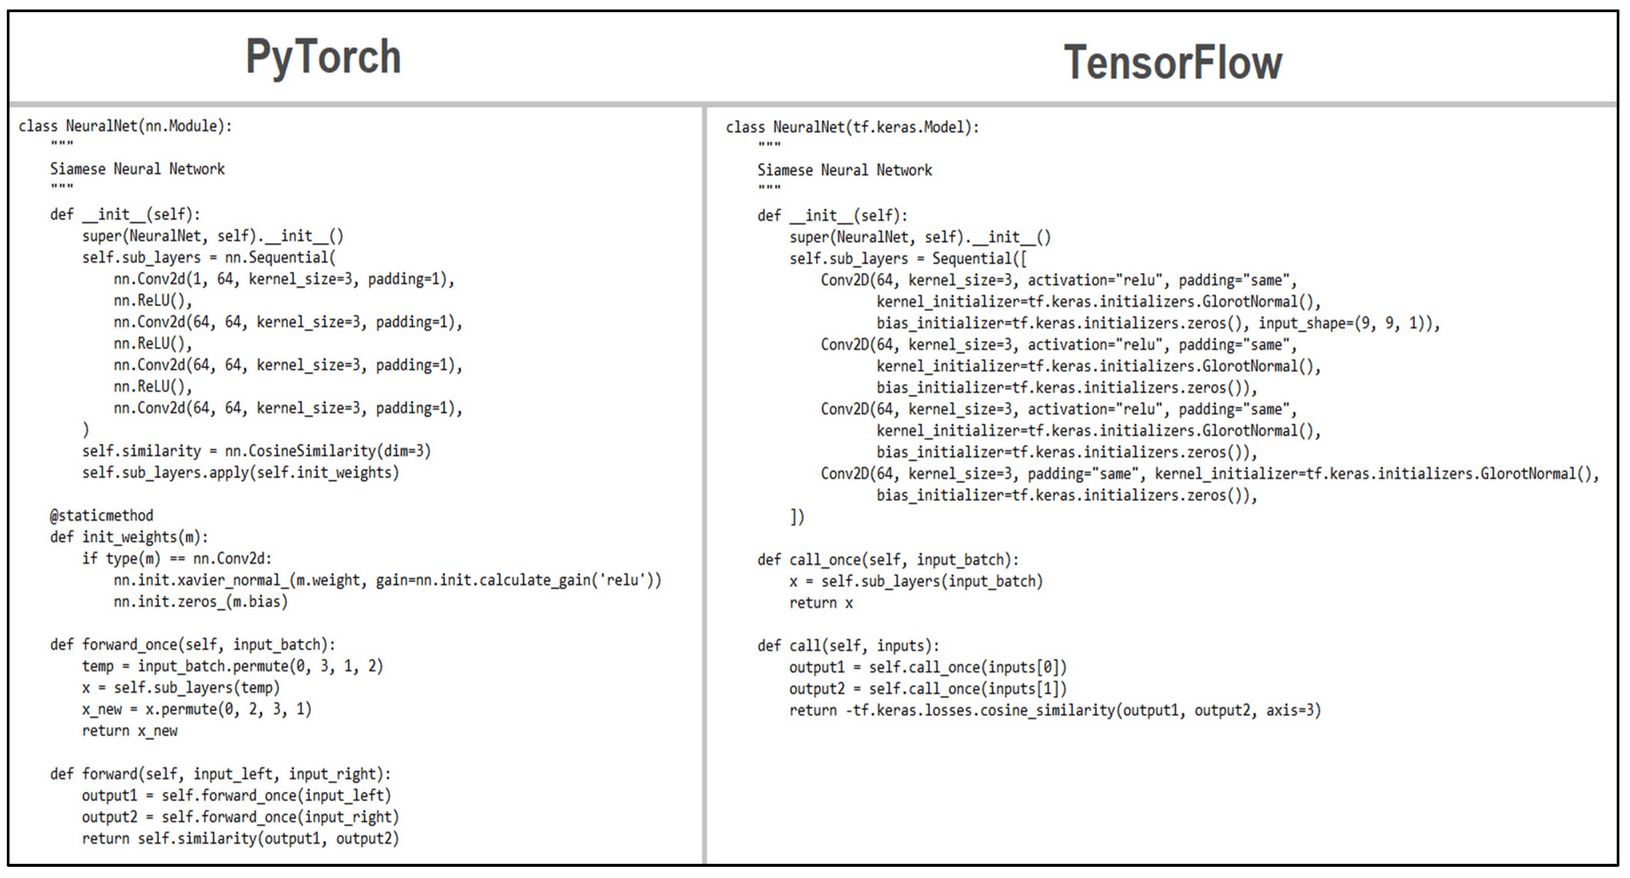
\includegraphics[scale=0.125]{figure1.png}
  \caption{\textsc{Comparison of Network Architectures}}
\end{figure}


In the image above, an architecture is defined using both PyTorch and TensorFlow. Both frameworks offer powerful tools for developing and implementing deep learning models but exhibit structural and functional differences. These differences can lead developers to make a choice based on their preferences, project requirements, and performance expectations.

In PyTorch, the model is defined as a class based on \texttt{nn.Module}. This structure provides flexibility and customizability while also offering a lower-level control option. In the PyTorch code, the layers forming the network are grouped using \texttt{nn.Sequential}, and each layer is explicitly defined. A helper method (\texttt{init\_weights}) is used to initialize the corresponding weights. Additionally, methods such as \texttt{forward} and \texttt{forward\_once} explicitly control the flow of operations on the model inputs. The \texttt{forward\_once} method, in particular, supports the Siamese network structure by using the same sub-layers for both inputs. This facilitates weight sharing and efficient computation. PyTorch’s approach is especially suitable for research and experimental work, as it gives developers full control over the model architecture. Thanks to the dynamic computation graph, the flow of the model is determined at runtime, making debugging and understanding the model's behavior easier.

On the other hand, in TensorFlow, the model is defined based on \texttt{tf.keras.Model}, offering a more user-friendly approach. The layers are listed within a \texttt{Sequential} object, and weight initialization is specified directly via the layer parameters. Unlike PyTorch, TensorFlow uses \texttt{call\_once} and \texttt{call} methods, which define operations in a more abstract and modular way. The \texttt{call\_once} method, similar to PyTorch’s \texttt{forward\_once} method, applies the same operations for both inputs. The \texttt{call} method takes the inputs, computes the outputs using the \texttt{call\_once} method, and then calculates the cosine similarity loss. TensorFlow's approach is especially suited for rapid prototyping and transitioning to production environments. The Keras API provides a high-level interface that simplifies model creation and allows for more complex models to be developed with less code. Due to the static computation graph, the model can be optimized and function more efficiently in distributed environments.

One key difference is the weight initialization process, which is implemented manually in PyTorch while it is more integrated in TensorFlow. In PyTorch, functions such as \texttt{nn.init.xavier\_normal\_} are used, whereas in TensorFlow, the weight initialization strategy is determined via the \texttt{kernel\_initializer} parameter. Additionally, while TensorFlow directly provides the \texttt{cosine\_similarity} loss, PyTorch performs this operation through a separate layer. This results in more concise code in TensorFlow. While PyTorch offers greater flexibility, TensorFlow provides a more structured experience in terms of ease of use. These differences may influence developers' choice of framework depending on the needs of the project. For example, PyTorch may be more suitable for research-focused projects and customized model architectures, while TensorFlow may be more appealing for rapid prototyping, easy deployment, and industrial applications. Both frameworks have their own unique advantages and disadvantages, and the right choice depends on the specific requirements of the project.


\begin{figure}[htbp]
  \centering
 %\usepackage[turkish]{babel} kullanıldığı için komuta gerek var
  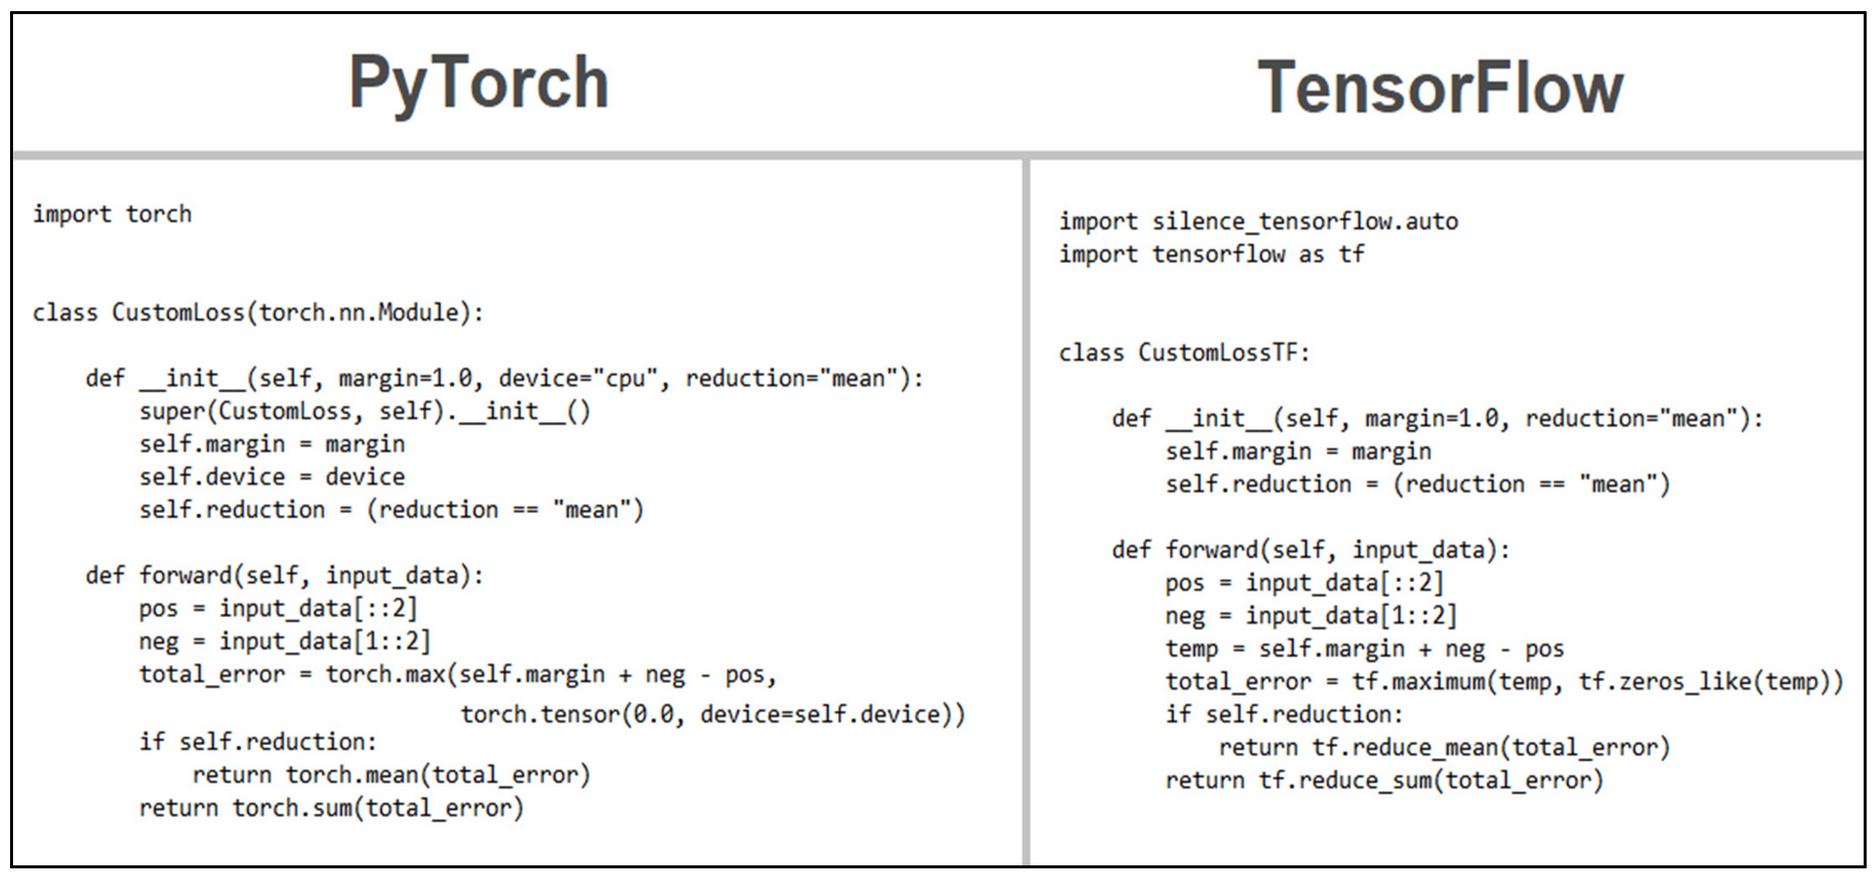
\includegraphics[scale=0.125]{figure2.png} % Dosya adı doğru olmalı
%\usepackage[turkish]{babel} kullanıldığı için komuta gerek var
\caption{\textsc{Comparison of Loss Functions}}
\end{figure}

In the PyTorch framework, the custom loss function is created through inheritance from the \texttt{torch.nn.Module} class. This reflects PyTorch's modular structure and enables the loss function to behave like a neural network layer. The \texttt{\_\_init\_\_} method defines the initial parameters of the loss function. Here, the \texttt{margin}, \texttt{device} (indicating whether the operations are carried out on the CPU or GPU), and \texttt{reduction} (indicating how the loss value will be aggregated, i.e., whether the mean or sum will be used) parameters are defined. The use of \texttt{self.device} ensures that tensors are created on the correct device and that operations are performed efficiently. The \texttt{forward} method is where the actual loss computation takes place. The input data is divided into \texttt{pos} (positive examples) and \texttt{neg} (negative examples). The loss is calculated using the expression \texttt{torch.max(self.margin + neg - pos, torch.tensor(0.0, device=self.device))}. This expression represents a variation of the "hinge loss" function. If the value of \texttt{self.margin + neg - pos} is greater than 0, this value is used; otherwise, 0 is used. Depending on the \texttt{reduction} parameter, the loss value is aggregated using \texttt{torch.mean} (mean) or \texttt{torch.sum} (sum). This approach in PyTorch provides greater flexibility and control over the loss function. For example, it is possible to use different layers or operations within the loss function.

In TensorFlow, the custom loss function is defined as a simpler Python class. Inheritance from the \texttt{tf.keras.losses.Loss} class is not used, offering a lighter structure. The \texttt{\_\_init\_\_} method takes \texttt{margin} and \texttt{reduction} parameters, similar to PyTorch, but lacks a \texttt{device} parameter, as TensorFlow generally adopts a more abstract approach to hardware management. The \texttt{forward} method operates similarly to the logic in PyTorch. The input data is divided into \texttt{pos} and \texttt{neg}, and the loss is computed using the expression \texttt{tf.maximum(temp, tf.zeros\_like(temp))}. Here, \texttt{temp = self.margin + neg - pos}. The \texttt{tf.maximum} function returns the maximum of the two values, analogous to \texttt{torch.max} in PyTorch. The \texttt{tf.zeros\_like(temp)} function creates a tensor with the same shape as \texttt{temp} but with all elements set to 0. Depending on the \texttt{reduction} parameter, the loss is aggregated using \texttt{tf.reduce\_mean} or \texttt{tf.reduce\_sum}. TensorFlow's approach allows for defining custom loss functions more quickly with less code.

In summary, both frameworks support the definition of custom loss functions. PyTorch offers more customization and flexibility with its \texttt{torch.nn.Module} infrastructure and low-level device control, while TensorFlow provides a more user-friendly and faster experience with a simpler class structure and high-level APIs. PyTorch's dynamic computation graph facilitates easier debugging and understanding of operations within the loss function, while TensorFlow's static computation graph can help optimize performance. The choice of framework for developers will depend on project requirements, experience levels, and performance expectations.


\begin{figure}[htbp]
  \centering
 %\usepackage[turkish]{babel} kullanıldığı için komuta gerek var
  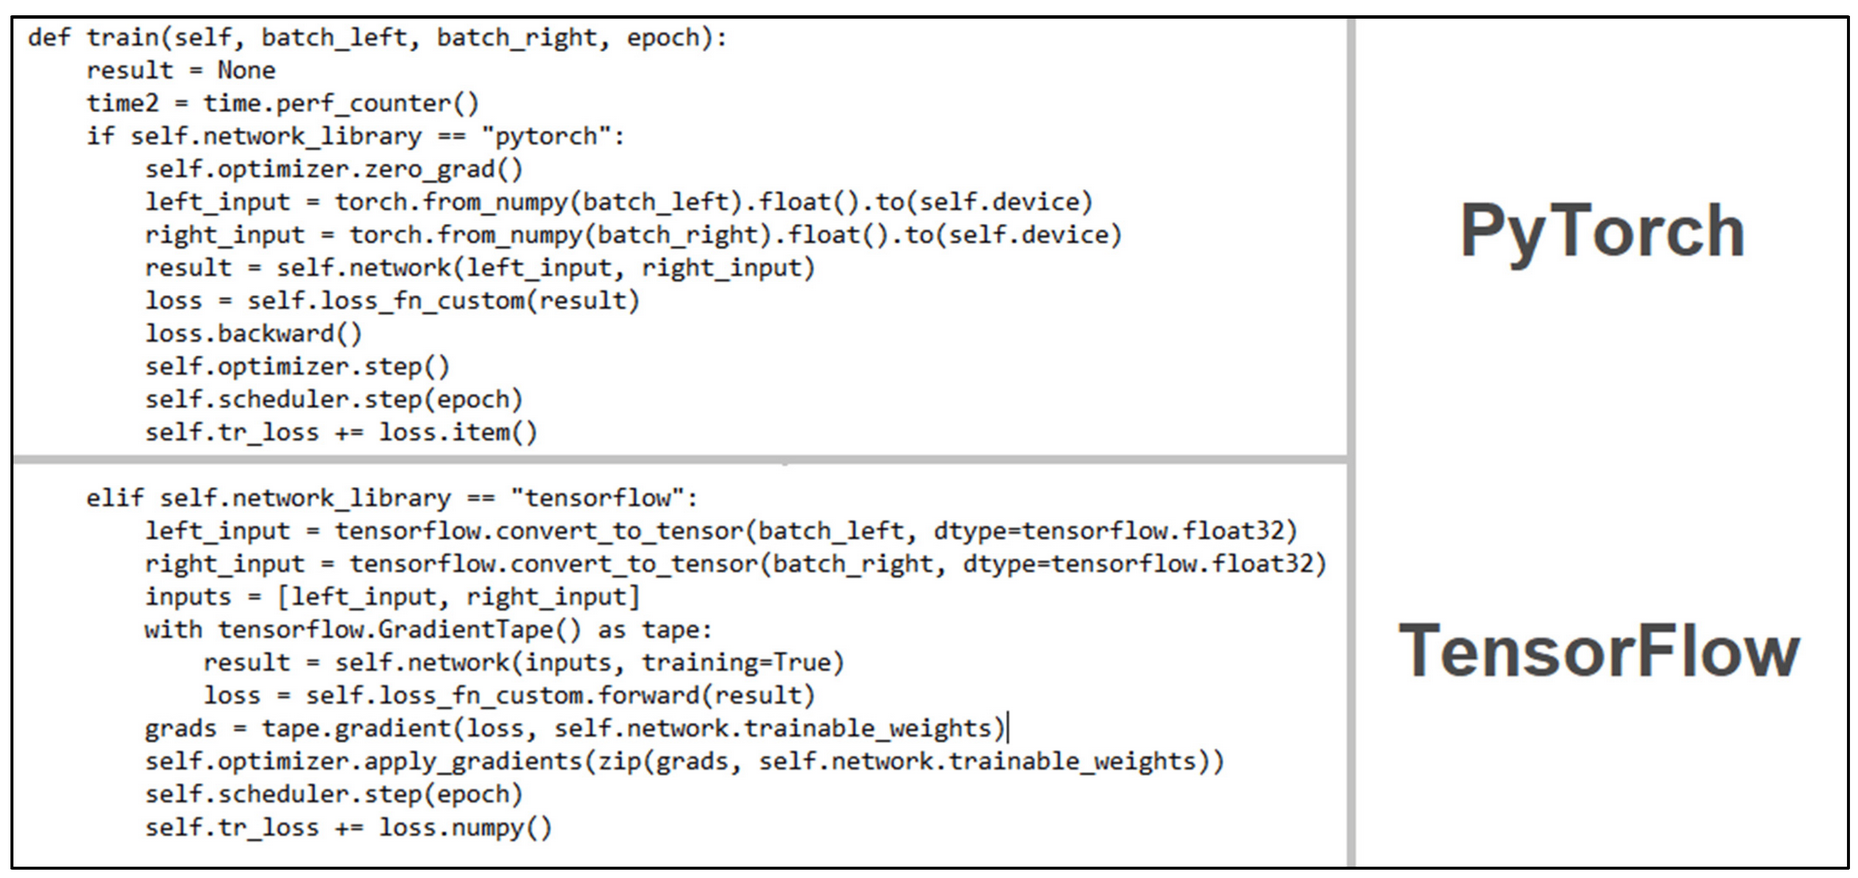
\includegraphics[scale=0.125]{figure3.png} % Dosya adı doğru olmalı
%\usepackage[turkish]{babel} kullanıldığı için komuta gerek var
\caption{\textsc{Training Flow}} 
\end{figure}

In PyTorch, the training loop provides a flexible structure for controlling optimization steps and data flow. The \texttt{train} function converts input data from \texttt{Numpy} arrays to PyTorch tensors using \texttt{torch.from\_numpy} and moves the data to the appropriate device (CPU or GPU) with the \texttt{to(self.device)} method. This is crucial for effectively utilizing hardware acceleration. PyTorch directly calls the \texttt{forward} method with \texttt{self.network(left\_input, right\_input)} to obtain the model’s output and applies the custom loss function with \texttt{self.loss\_fn\_custom(result)}. Gradients are computed using the automatic differentiation mechanism with the \texttt{loss.backward()} method. The optimization step is carried out with \texttt{self.optimizer.step()}, which updates the model’s weights using the calculated gradients. To update hyperparameters such as the learning rate, the \texttt{self.scheduler.step(epoch)} method is used, allowing the learning rate to be dynamically adjusted throughout the training process. The loss value is converted to a Python number with \texttt{loss.item()} and added to the \texttt{self.tr\_loss} variable to facilitate tracking the training progress. This approach in PyTorch gives developers more detailed control over the training loop and makes it easier to implement customized training strategies. Notably, the dynamic computation graph allows for modifying the model structure during training, which is a significant advantage for researchers and experimental work.

In contrast, TensorFlow adopts a more structured and user-friendly approach to the training loop. Data transformations are performed using \texttt{tensorflow.convert\_to\_tensor}, converting the data into TensorFlow tensors. Gradient calculations and optimization are encapsulated within the \texttt{with tensorflow.GradientTape() as tape:} context manager. All operations performed within this block are recorded and used for gradient computation. The model’s output is obtained with \texttt{result = self.network(inputs, training=True)}, where the \texttt{training=True} argument ensures the model operates in training mode, activating layers like \texttt{Dropout}. The loss function is computed using \texttt{loss = self.loss\_fn\_custom.forward(result)}. Gradients are automatically computed with \texttt{tape.gradient(loss, self.network.trainable\_weights)}, where \texttt{self.network.trainable\_weights} includes the model’s trainable weights. The optimization step is performed with \texttt{self.optimizer.apply\_gradients(zip(grads, self.network.trainable\_weights))}, applying the computed gradients to the model’s weights. Learning rate updates are also handled using \texttt{self.scheduler.step(epoch)}. Loss values are converted from TensorFlow tensors to Numpy arrays using \texttt{loss.numpy()} and added to the \texttt{self.tr\_loss} variable. TensorFlow’s approach enables the creation of cleaner and more readable training loops with less code. The static computation graph also allows the model to be optimized and work more efficiently in distributed environments.

While PyTorch offers a more suitable solution for cases requiring low-level control and customization, TensorFlow’s context managers and integrated methods support ease of use and a cleaner code structure. Both frameworks have their unique advantages and disadvantages, and the correct choice depends on the project requirements. Furthermore, Liang et al. (2019) noted that TensorFlow’s advanced optimization in automatic differentiation algorithms provides performance advantages for more complex models in certain cases. However, PyTorch’s Python-centric design offers developers a more intuitive programming environment[15]. This intuitiveness is particularly beneficial when working with complex models such as dynamic neural networks.


\renewcommand{\tablename}{Table}  % Tablo yerine Table yazılmasını sağlıyoruz

\begin{table}[h!]
\centering
\caption{\textsc{PyTorch and TensorFlow Time Comparison}}
\renewcommand{\arraystretch}{1} % Satır aralığını azaltır
\setlength{\tabcolsep}{3pt} % Sütunlar arası boşluğu azaltır
\begin{tabular}{|l|c|c|}
\hline
\textbf{\textsc{Measurement}}          & \textbf{\textsc{PyTorch Time}} & \textbf{\textsc{TensorFlow Time}} \\ \hline
Total training time                     & 16 h 58 m 51.032 s            & 21 h 56 m 53.515 s                \\ \hline
Average epoch time                      & 1 h 10 m 48.891 s             & 1 h 32 m 6.028 s                  \\ \hline
Network \& Optimization time            & 0.000869 s                    & 0.0011189 s                       \\ \hline
Execution time                          & 1.1743711 s                   & 2.6666322 s                       \\ \hline
\end{tabular}
\end{table}


To explain the table above:  
"Total training time" represents the total duration required for the network to be fully trained on the given dataset. This metric reflects the total time spent training the model on all training data for multiple passes (for as many epochs as specified) and serves as an important indicator of the model's overall training performance. "Average epoch time" refers to the time taken for the network to process the training set once. This indicates the duration of each epoch and is used to assess the stability and efficiency of the training process. "Network and Optimization time" defines the time taken to complete the optimization stage from the initial input. This metric encompasses the forward pass, loss calculation, backward pass, and weight update steps. A lower time value in this category indicates the efficiency with which the framework applies its optimization algorithms. "Execution time" refers to the real-time duration required to reach a result during evaluation. This is the time taken by the trained model to generate predictions on new data, which is a critical metric for real-time applications.

When comparing PyTorch's total training time (\textit{16 hours 58 minutes 51 seconds}) with TensorFlow's total training time (\textit{21 hours 56 minutes 53 seconds}), it is observed that PyTorch completes the training approximately \%22 faster. This result indicates that PyTorch offers a faster model training process. In terms of average epoch time, PyTorch (\textit{1 hour 10 minutes 48 seconds}) demonstrates more efficient performance compared to TensorFlow (\textit{1 hour 32 minutes 6 seconds}). This shows that each training cycle is completed more quickly with PyTorch. Regarding network and optimization time, both frameworks exhibit very low time values. However, PyTorch's optimization time (\textit{0.000869 seconds}) is \%22 shorter than TensorFlow's (\textit{0.0011189 seconds}). This indicates that PyTorch computes gradients and updates weights more efficiently. When considering execution time, PyTorch's execution time (\textit{1.1743711 seconds}) is \%56 shorter than TensorFlow's (\textit{2.6666322 seconds}). This suggests that model predictions can be made faster with PyTorch in real-time applications. This difference may be attributed to PyTorch's more optimized tensor operations and execution engine. In particular, PyTorch's "Just-In-Time" (JIT) compiler can help improve execution speed.

These findings suggest that PyTorch is a more advantageous choice, particularly for projects that have speed requirements and involve large-scale datasets. For example, in real-time image processing or natural language processing applications, where low execution time is critical, PyTorch may be a more appropriate choice. Additionally, the \%22 reduction in total training time can result in significant time savings when training on large datasets. However, TensorFlow also has its own unique advantages. In particular, TensorFlow may offer stronger capabilities for distributed training, integration into production environments, and mobile deployment. Therefore, the selection of the framework should be based on the project's specific requirements and priorities. If speed is a critical factor, PyTorch may be a more appealing option, while TensorFlow may be more suitable if scalability and production-oriented features are prioritized.


\section{Algorithm}

The field of data science has rapidly evolved with a variety of specialized tools and frameworks that support processes such as data processing, modeling, optimization, and deployment. Popular frameworks like TensorFlow and PyTorch have revolutionized the development and training of complex neural networks in deep learning. Similarly, Scikit-learn provides a user-friendly structure for traditional machine learning tasks, while tools like Pandas and NumPy facilitate data preprocessing and transformation. These tools have enabled data scientists and machine learning engineers to efficiently carry out various tasks, significantly contributing to advancements in the field. Notably, TensorFlow and PyTorch’s GPU acceleration and distributed training capabilities have made it possible to train complex models on large datasets. Scikit-learn, with its simple and intuitive interface, has served as an important entry point for those new to machine learning. Pandas and NumPy, on the other hand, have become fundamental tools for data manipulation and numerical computations.

However, the current data science ecosystem is fragmented due to the need for different tools at each stage of the process. This fragmentation leads to inefficiencies such as integration challenges, code duplication, and complex workflows. For instance, in a data science project, one may need to use Pandas for data preprocessing, Scikit-learn or TensorFlow/PyTorch for model training, different metric libraries for model evaluation, and separate tools for model deployment. Converting data formats between these various tools, resolving compatibility issues, and managing workflows can be a time-consuming and error-prone process. Furthermore, switching between different tools requires developers to learn various APIs and usage methods, which increases the learning curve and reduces productivity. This fragmented structure also leads to reproducibility issues, as achieving consistent results across different environments becomes challenging.

These shortcomings clearly highlight the need for an integrated platform that consolidates data science processes from start to finish. Such a platform, by encompassing all steps from data acquisition to model deployment, can help data scientists and machine learning engineers streamline and accelerate their workflows. The EmreAI Framework has been developed to meet this need. By combining all stages from data acquisition to model deployment, this framework simplifies and accelerates workflows. With its modular architecture, EmreAI provides a flexible structure that brings together the strengths of existing tools while addressing significant gaps. Integrated frameworks like EmreAI can shorten the development time of data science projects, reduce code duplication, eliminate integration issues, and lead to more efficient and consistent outcomes. Such an approach can contribute to making data science a more accessible and efficient field. Additionally, frameworks like EmreAI can offer automatic machine learning (AutoML) capabilities, making it easier for non-expert users to create and deploy machine learning models.

\subsection{Introduction to Algorithm}

The current data science ecosystem consists of numerous tools and libraries, each focused on a specific task. While this provides a wealth of options for data scientists, it also leads to integration challenges and inefficiencies. This fragmented structure requires data scientists to convert data formats between different tools, solve compatibility issues, and manage complex workflows, resulting in time and resource waste. 

\begin{itemize}
    \item \textbf{Data Preprocessing:} Libraries such as Pandas, NumPy, and Scikit-learn are used for data cleaning, transformation, and feature engineering. However, scalability issues may arise when working with large datasets. Pandas is optimized primarily for in-memory operations, and performance problems may occur when very large datasets do not fit into RAM. In such cases, distributed processing frameworks like Spark or Dask may be required, which adds complexity.
    
    \item \textbf{Model Training:} TensorFlow and PyTorch provide powerful tools for deep learning models, but are less suitable for traditional machine learning algorithms. Scikit-learn offers a more user-friendly interface in this area but has limited capabilities for deep learning models and distributed training. This situation necessitates the use of different frameworks for various model types, leading to code duplication and integration challenges. For example, if both deep learning and traditional machine learning models are required in a project, switching between two different frameworks and converting data formats may be necessary.
    
    \item \textbf{Hyperparameter Optimization:} Tools such as Optuna, Ray Tune, and Hyperopt automate the hyperparameter search process. However, the integration and management of these tools require additional effort. These tools are generally designed to be integrated with specific model training frameworks (e.g., Scikit-learn, TensorFlow, or PyTorch), and compatibility issues may arise when used alongside different frameworks. Additionally, the use of these tools requires the correct definition of the search space and the selection of appropriate search algorithms, which is an expert-level task.
    
    \item \textbf{Model Deployment:} Tools like TensorFlow Serving, TorchServe, and Flask are used for deploying trained models. However, the setup and configuration of these tools can be complex. These tools often support specific model formats (e.g., SavedModel or ONNX), and format conversion processes may be necessary when deploying models trained in different frameworks. Moreover, scalability, security, and monitoring concerns must also be considered when using these tools.
\end{itemize}

In summary, EmreAI allows users to perform all tasks within the platform without having to switch between separate tools like Pandas, TensorFlow, or Flask. This feature resolves incompatibilities in workflows, saves time, and accelerates project processes. Integrated platforms like EmreAI simplify data science processes, enabling data scientists and machine learning engineers to be more productive and helping projects to be completed more quickly and efficiently. Furthermore, such platforms can provide more comprehensive and effective solutions by combining the strengths of different tools. For instance, EmreAI can support both traditional machine learning algorithms and deep learning models, automate hyperparameter optimization, and streamline model deployment.

\subsection{Tool Definition}

\subsubsection{Key Features}

\begin{itemize}
    \item \textbf{Unified Workflow Integration:} EmreAI presents all steps, from data acquisition to model deployment, in an integrated manner. This eliminates the need for data scientists to switch between different tools and significantly simplifies the workflow. EmreAI offers a modular structure through an orchestration layer, automating steps such as data acquisition, preprocessing, model training, optimization, evaluation, and deployment. Modules are available for connecting to different data sources (databases, cloud storage, APIs, etc.), and these modules convert the data into a standard format before passing it to subsequent steps.

    \item \textbf{Modular Design:} EmreAI's architecture treats each step (data preprocessing, modeling, optimization, deployment) as independent modules. This modularity ensures flexibility, reusability, and easy extensibility. Each function (e.g., feature engineering, model selection, hyperparameter optimization) is implemented as an independent module. Modules communicate through standard interfaces and can be easily modified or updated. As a result, when new algorithms or techniques are added, significant changes to the overall system are not required.

    \item \textbf{Hybrid Backend Support:} EmreAI can run on both CPU and GPU, leveraging GPU acceleration through integration with libraries such as CUDA and cuDNN. Additionally, it offers automatic scaling and resource management capabilities through integration with cloud platforms (AWS, GCP, Azure). Cloud integration is achieved via the APIs of cloud platforms, allowing users to train and deploy models on the platform and hardware of their choice.

    \item \textbf{AutoML and Hyperparameter Tuning:} EmreAI includes a built-in AutoML engine featuring advanced hyperparameter optimization algorithms (Bayesian optimization, genetic algorithms, Population-Based Training (PBT)). This engine automatically explores different hyperparameter combinations to find the best model performance. The AutoML engine tests various hyperparameter combinations within the specified search space, performing model training for each combination. Bayesian optimization uses the results of previous trials to select better combinations for subsequent trials. Genetic algorithms employ a population-based approach, while PBT trains multiple models concurrently and periodically copies the hyperparameters of the best-performing models to others.

    \item \textbf{Reproducibility and Experiment Management:} EmreAI can integrate with tools like MLflow to ensure the reproducibility of experiments and results. This makes it easier to record, compare, and reproduce experiments. Furthermore, integration with DVC (Data Version Control) allows for data and model versioning. Through MLflow integration, the parameters, metrics, code version, and artifacts of each experiment are recorded. DVC integration ensures the versioning of datasets and models.

    \item \textbf{Deployment-Ready APIs:} EmreAI simplifies the creation of RESTful APIs for trained models, making it easier to integrate models into web applications, mobile applications, or other systems.

    \item \textbf{Explainable AI (XAI):} EmreAI integrates XAI techniques such as SHAP, LIME, and Grad-CAM, enabling the understanding of how model predictions are made. This improves model reliability and enhances transparency in decision-making processes.

    \item \textbf{Scalable Data Management:} To efficiently work with large datasets, EmreAI utilizes technologies such as Apache Arrow and Parquet. Furthermore, it can scale data processing and model training through integration with distributed computing frameworks like Dask or Spark.
\end{itemize}


\subsubsection{Architecture}

EmreAI's architecture consists of the following layers:

\begin{itemize}

    \item \textbf{Data Access Layer:} This layer provides access to various data sources such as CSV, JSON, Parquet, SQL databases, and cloud storage services (AWS S3, Google Cloud Storage, Azure Blob Storage). Data reading and writing operations are optimized using libraries such as Apache Arrow and Pandas.

    The system can connect to various data sources, including CSV, JSON, Parquet files, SQL databases (MySQL, PostgreSQL, etc.), and cloud storage services (AWS S3, Google Cloud Storage, Azure Blob Storage). Data reading and writing operations are optimized using libraries like Apache Arrow and Pandas, ensuring high-performance data access. For example, when reading a large CSV file, Apache Arrow improves the read speed by more efficiently representing the data in memory.
    
    \item \textbf{Data Processing Layer:} This layer performs tasks such as data cleaning, transformation, feature engineering, and feature selection. Scikit-learn and custom algorithms are used in this layer. Distributed data processing capabilities are provided through Dask integration for handling large datasets.
    
    \item \textbf{Modeling Layer:} This layer facilitates the creation and training of machine learning and deep learning models. Libraries such as TensorFlow, PyTorch, and Scikit-learn are integrated into this layer. Users can either use high-level APIs provided by EmreAI or directly leverage these libraries to create custom models.
    
    Commonly used machine learning and deep learning libraries like TensorFlow, PyTorch, and Scikit-learn are integrated into the system. Users can quickly build models using the high-level APIs offered by EmreAI or develop more customized models using these libraries directly. For instance, TensorFlow or PyTorch may be used to train a neural network model, while Scikit-learn can be used for more traditional machine learning algorithms.
    
    \item \textbf{Optimization Layer:} This layer handles tasks such as hyperparameter optimization, model selection, and model validation. Tools such as Optuna, Ray Tune, and Hyperopt are integrated into this layer. Additionally, MLflow integration is provided for experiment management and monitoring.
    
    Hyperparameters, such as learning rate, batch size, and the number of layers, significantly affect model performance. This layer utilizes tools like Optuna, Ray Tune, and Hyperopt to automatically identify the optimal values for these parameters. These tools offer various optimization algorithms, including Bayesian optimization, genetic algorithms, and random search.
    
    Different machine learning algorithms (e.g., linear regression, support vector machines, random forests, neural networks) perform differently on various datasets. This layer tests various algorithms and selects the best-performing model.
    
    Techniques like k-fold cross-validation are used to assess the model’s generalization ability. This helps to prevent overfitting by evaluating how well the model performs on different subsets of data.
    
    \item \textbf{Deployment Layer:} This layer facilitates the deployment and management of trained models. The support for ONNX format enables exporting models to different platforms. RESTful APIs can be created using web frameworks like Flask or FastAPI. Additionally, integration with Docker and Kubernetes offers containerized deployment options.
    
    \item \textbf{Explainability Layer:} This layer applies Explainable AI (XAI) techniques to understand how model predictions are made. Libraries such as SHAP, LIME, and Grad-CAM are integrated into this layer.
    
    LIME approximates a complex model with a simpler model (e.g., a linear model) to explain the predictions of the model. This helps to understand how the model made a decision for a particular data point. For instance, in an image classification model, LIME can show which pixels the model focused on when classifying an image.
    
    Grad-CAM, particularly used in image classification models, generates a heatmap to show which regions the model focused on while classifying an image. This helps to understand what the model "sees" visually. For example, in an object detection model, Grad-CAM highlights where the model identified the object.
    
\end{itemize}



\subsubsection{Workflow Example}
The following Python code demonstrates how to create a machine learning workflow using the EmreAI library. This example includes steps for data loading and preprocessing, model training, and hyperparameter optimization:

Below is an example showing how to create a machine learning workflow using the EmreAI library. In this example, steps for data loading, preprocessing, model training, and hyperparameter optimization are provided.

\begin{figure}[htbp]
  \centering
  %\usepackage[turkish]{babel} requires this command
  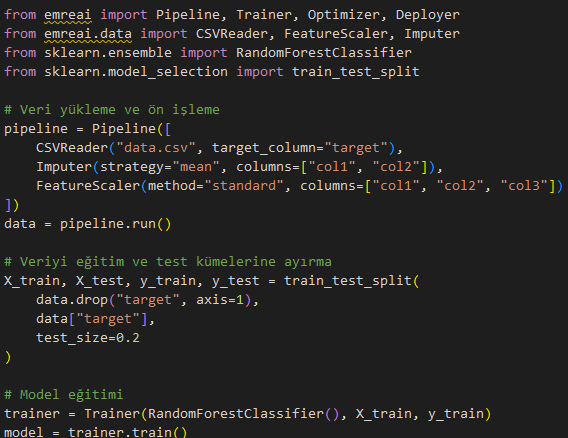
\includegraphics[scale=0.550]{figure4.png} % Ensure the file name is correct
%\usepackage[turkish]{babel} requires this command
\caption{\textsc{Data Loading and Training}}

\end{figure}

\paragraph{Library Imports}

\begin{itemize}
    \item \textbf{Core Components:} The classes \texttt{Pipeline}, \texttt{Trainer}, \texttt{Optimizer}, and \texttt{Deployer} are imported from the \texttt{emreai} library.
    \begin{itemize}
        \item \texttt{Pipeline}: Used to apply data preprocessing steps sequentially.
        \item \texttt{Trainer}: Used to train the machine learning model.
        \item \texttt{Optimizer}: Used for hyperparameter optimization of the model (not directly used in the code).
        \item \texttt{Deployer}: Used for deploying the trained model.
    \end{itemize}
    \item \textbf{Data Processing Modules:} The classes \texttt{CSVReader}, \texttt{FeatureScaler}, and \texttt{Imputer} are imported from the \texttt{emreai.data} module.
    \begin{itemize}
        \item \texttt{CSVReader}: Used to read data in CSV format.
        \item \texttt{FeatureScaler}: Used for scaling data.
        \item \texttt{Imputer}: Used for imputation (filling missing values).
    \end{itemize}
\end{itemize}

\begin{itemize}
    \item \textbf{Model and Data Splitting:}
    \begin{itemize}
        \item \texttt{RandomForestClassifier}: The Random Forest classification algorithm is imported from the \texttt{sklearn.ensemble} module. This will be the main machine learning model used in the project.
        \item \texttt{train\_test\_split}: The function to split the dataset into training and testing sets is imported from the \texttt{sklearn.model\_selection} module.
    \end{itemize}
\end{itemize}

\paragraph{Data Loading and Preprocessing}

A \texttt{Pipeline} object is created, which defines the sequence of steps to be applied to the data.

\begin{itemize}
    \item \texttt{CSVReader("data.csv", target\_column="target")}: Reads the \texttt{"data.csv"} file. The \texttt{target\_column} parameter specifies the name of the target variable (the column to be predicted).
    \item \texttt{Imputer(strategy="mean", columns=["col1", "col2"])}: Fills missing values in the \texttt{"col1"} and \texttt{"col2"} columns with their mean values. The \texttt{strategy} parameter defines the imputation method (\texttt{"mean"} for the mean, \texttt{"median"} for the median, or \texttt{"most\_frequent"} for the most frequent value).
    \item \texttt{FeatureScaler(method="standard", columns=["col1", "col2", "col3"])}: Standardizes the \texttt{"col1"}, \texttt{"col2"}, and \texttt{"col3"} columns (Z-score normalization). This makes the mean of each feature 0 and the standard deviation 1. The \texttt{method} parameter can accept other scaling methods such as \texttt{"minmax"} (scaling to the range 0-1).
\end{itemize}


\begin{figure}[htbp]
  \centering
 %\usepackage[turkish]{babel} kullanıldığı için komuta gerek var
  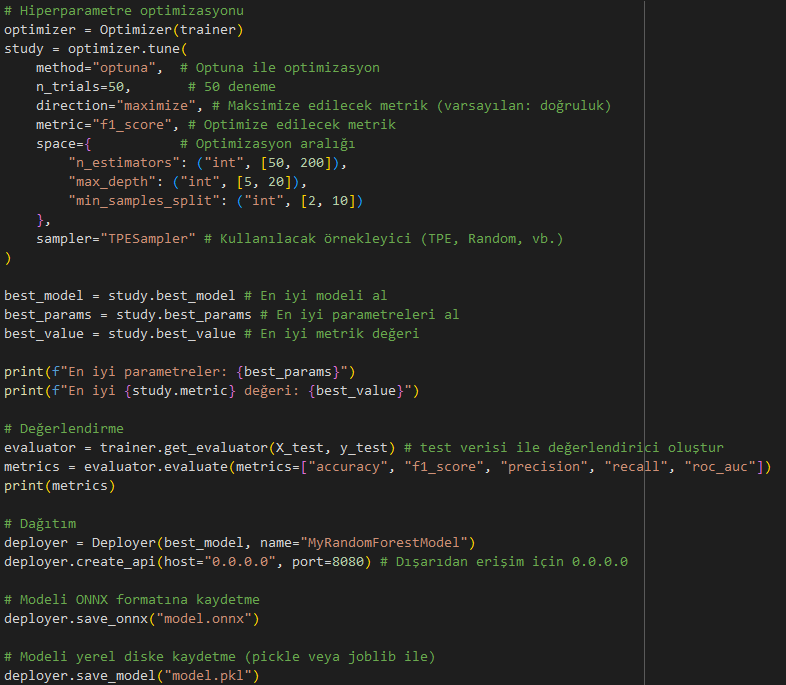
\includegraphics[scale=0.500]{figure5.png} % Dosya adı doğru olmalı
 %\usepackage[turkish]{babel} kullanıldığı için komuta gerek var
\caption{\textsc{Hyperparameter Optimization}}
\end{figure}

\paragraph{Hyperparameter Optimization}

\begin{itemize}
    \item \texttt{optimizer = Optimizer(trainer)}: The \texttt{Optimizer} class is initialized with the trained \texttt{trainer} object. This specifies the model on which the optimization process will be performed.
    \item \texttt{study = optimizer.tune(...)}: Initiates the optimization process. The \texttt{tune()} method supports various optimization strategies.
    \begin{itemize}
        \item \texttt{method="optuna"}: Specifies that the Optuna library will be used for optimization. Optuna is a popular framework for automatic hyperparameter optimization.
        \item \texttt{n\_trials=50}: Specifies that the optimization will be conducted with 50 different trials (iterations). In each trial, different hyperparameter combinations are tested.
        \item \texttt{direction="maximize"}: Specifies that the optimization aims to maximize the given metric (in this case, the "f1\_score"). For different optimization problems, \texttt{"minimize"} can also be used.
        \item \texttt{metric="f1\_score"}: Specifies the metric to be optimized during the process. The F1 score is the harmonic mean of precision and recall and is a better measure than accuracy for imbalanced datasets.
        \item \texttt{space=\{...\}}: Defines the range of hyperparameters to be searched during optimization.
        \begin{itemize}
            \item \texttt{"n\_estimators": ("int", [50, 200])}: Specifies that the number of trees in the Random Forest model will take integer values between 50 and 200.
            \item \texttt{"max\_depth": ("int", [5, 20])}: Specifies that the maximum depth of the trees will take integer values between 5 and 20.
            \item \texttt{"min\_samples\_split": ("int", [2, 10])}: Specifies that the minimum number of samples required to split a node will take integer values between 2 and 10.
        \end{itemize}
        \item \texttt{sampler="TPESampler"}: Specifies the sampling algorithm used by Optuna. The \texttt{TPESampler} (Tree-structured Parzen Estimator) is an advanced sampler based on Bayesian optimization, providing a more efficient search compared to random sampling.
    \end{itemize}
    \item \texttt{best\_model = study.best\_model}: Assigns the best model found during optimization to the \texttt{best\_model} variable.
    \item \texttt{best\_params = study.best\_params}: Assigns the hyperparameters of the best model as a dictionary to the \texttt{best\_params} variable.
    \item \texttt{best\_value = study.best\_value}: Assigns the metric value obtained by the best model (in this case, the F1 score) to the \texttt{best\_value} variable.
    \item \texttt{print(f"Best parameters: \{best\_params\}")}: Prints the best hyperparameters to the screen.
    \item \texttt{print(f"Best \{study.metric\} value: \{best\_value\}")}: Prints the best metric value to the screen.
\end{itemize}

\paragraph{Model Evaluation}

\begin{itemize}
    \item \texttt{evaluator = trainer.get\_evaluator(X\_test, y\_test)}: Creates an evaluator object with the test data (\texttt{X\_test}, \texttt{y\_test}). This object is used to measure the model's performance on the test data.
    \item \texttt{metrics = evaluator.evaluate(}\\
    \texttt{metrics=["accuracy", "f1\_score", "precision",}\\
    \texttt{"recall", "roc\_auc"])}: Evaluates the model's performance based on the specified metrics.

    \begin{itemize}
        \item \texttt{accuracy}: Accuracy is the ratio of correct predictions to total predictions.
        \item \texttt{f1\_score}: The F1 score is the harmonic mean of precision and recall.
        \item \texttt{precision}: Precision is the ratio of true positive predictions to all positive predictions.
        \item \texttt{recall}: Recall is the ratio of true positive predictions to all actual positives.
        \item \texttt{roc\_auc}: The area under the ROC curve, which measures the model's classification performance.
    \end{itemize}
    \item \texttt{print(metrics)}: Prints the calculated metrics to the screen.
\end{itemize}

\paragraph{Model Deployment}

\begin{itemize}
    \item \texttt{deployer = Deployer(best\_model, name="MyRandomForestModel")}: Creates a deployment object with the best trained model and a name (\texttt{name}).
    \item \texttt{deployer.create\_api(host="0.0.0.0", port=8080)}: Creates a RESTful API for the model.
    \begin{itemize}
        \item \texttt{host="0.0.0.0"}: Ensures that the API is accessible from all network interfaces (local and external).
        \item \texttt{port=8080}: Specifies the port number on which the API will listen.
    \end{itemize}
    \item \texttt{deployer.save\_onnx("model.onnx")}: Saves the model in ONNX (Open Neural Network Exchange) format. ONNX is a standard for model exchange across different machine learning frameworks, allowing the model to be run on different platforms and languages.
    \item \texttt{deployer.save\_model("model.pkl")}: Saves the model to the local disk. This is typically done using Python's pickle or joblib libraries, enabling the model to be loaded later.
\end{itemize}


\section{EmreAI Model Deployment}

This section provides a detailed explanation of the process of deploying a machine learning model trained using the EmreAI framework. The goal is to ensure that users reading this section can successfully deploy their own models by following the described steps.

\subsection{Prerequisites}

Before starting with EmreAI, certain prerequisites need to be met:
\begin{itemize}
    \item \textbf{Python}: Python version 3.7 or higher must be installed on the system. The appropriate version can be downloaded from the official Python website (python.org).
\end{itemize}

\subsubsection{Environment Setup}

It is recommended to create a virtual environment to isolate project dependencies, preventing potential conflicts.  
The following commands should be used in the command line (terminal or command prompt):
\begin{itemize}
    \item \texttt{python3 -m venv emreai\_env}  \# macOS/Linux
    \item \texttt{python -m venv emreai\_env}    \# Windows
    \item \texttt{source emreai\_env/bin/activate}  \# macOS/Linux
    \item \texttt{emreai\_env\textbackslash Scripts\textbackslash activate}  \# Windows
\end{itemize}

Ensure that the EmreAI library and its dependencies (such as TensorFlow, PyTorch, Scikit-learn, Optuna, Flask/FastAPI, etc.) are correctly installed on your system.  
Installation instructions can be found in the EmreAI documentation. An example installation command is:
\texttt{pip install emreai scikit-learn pandas numpy tensorflow optuna mlflow dvc}

\subsection{Dataset Preparation}

To start a machine learning project with EmreAI, an appropriate dataset is required.  
For example, a simple CSV file will be used. A file named \texttt{"data.csv"} is created and populated with comma-separated data.  
The dataset includes a target variable (the column to be predicted) and features. In this example, a dataset containing missing values will be used.  
EmreAI can automatically handle these missing values.

In addition to CSV files, EmreAI can also process different types of data:
\begin{itemize}
    \item \textbf{Text Data:} Text data is used for natural language processing (NLP) tasks such as text classification, sentiment analysis, and text summarization. Text data is typically stored in files like .txt or .json.
    \item \textbf{Image Data:} Image data is used for tasks like image classification, object detection, and image segmentation. Image data is usually stored in files like .jpg, .png, or .jpeg.
    \item \textbf{Time Series Data:} Time series data is collected over a specific time period. Examples include stock prices, weather data, and sensor readings.
\end{itemize}

Start by importing the EmreAI modules and other libraries:
\begin{scriptsize}
\begin{verbatim}
from emreai import Pipeline, Trainer, Optimizer, Deployer
from emreai.data import CSVReader, FeatureScaler, Imputer
from sklearn.ensemble import RandomForestClassifier
from sklearn.model_selection import train_test_split
\end{verbatim}
\end{scriptsize}

In this step, a data processing pipeline is created using the \texttt{Pipeline} class. This pipeline defines how the data will be loaded and how preprocessing steps will be applied.

\begin{scriptsize}
\begin{verbatim}
pipeline = Pipeline([
    CSVReader("data.csv", target_column="target"),
    Imputer(strategy="mean", columns=["col1", "col2"]),
    FeatureScaler(method="standard", columns=["col1", 
    "col2", "col3"])
])

X, y = pipeline.run()  # Executes the pipeline
\end{verbatim}
\end{scriptsize}

\begin{itemize}
    \item \texttt{CSVReader}: Reads the CSV file and converts the data into a Pandas DataFrame. The \texttt{target\_column} parameter specifies the name of the target variable.
    \item \texttt{Imputer}: Used to fill missing values. The \texttt{strategy} parameter specifies the imputation method (\texttt{mean}, \texttt{median}, \texttt{most\_frequent}). The \texttt{columns} parameter indicates which columns will have their missing values filled.
    \item \texttt{FeatureScaler}: Used to scale the data. The \texttt{method} parameter specifies the scaling method (\texttt{standard}, \texttt{minmax}).
\end{itemize}

\subsubsection{Text Data Preprocessing}

\renewcommand{\figurename}{Figure}

\begin{figure}[htbp]
  \centering
  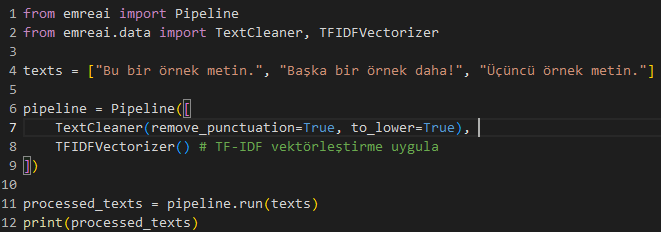
\includegraphics[scale=0.500]{figure9.png}
  \caption{\textsc{Text Data Preprocessing}}
\end{figure}


\textbf{TextCleaner:} Used for cleaning text data. The \texttt{remove\_punctuation} parameter removes punctuation marks, and the \texttt{to\_lower} parameter converts the text to lowercase. Additional parameters can be added (e.g., remove numbers, remove special characters).

\textbf{TFIDFVectorizer:} Converts text data into numerical representations (TF-IDF vectors).

Before training the model, the dataset must be split into training and testing sets to evaluate the model's generalization ability.

\begin{footnotesize}
\begin{verbatim}
X_train, X_test,
y_train, y_test = train_test_split(X,
y, test_size=0.2, random_state=42)
\end{verbatim}
\end{footnotesize}

\begin{itemize}
    \item The \texttt{train\_test\_split} function splits the data randomly according to the specified ratio (e.g., \texttt{0.2} for test data). The \texttt{random\_state} parameter sets a random seed for reproducibility.
\end{itemize}

\subsubsection{Image Data Preprocessing}

\begin{figure}[htbp]
  \centering
  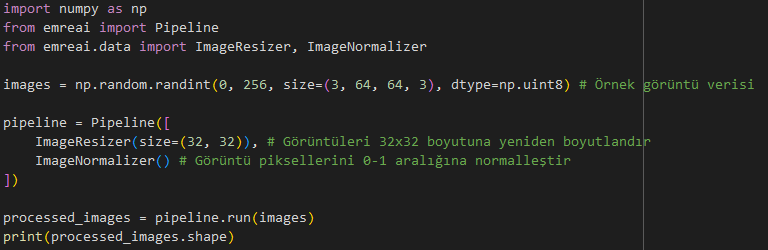
\includegraphics[scale=0.500]{figure10.png}
  \caption{\textsc{Image Data Preprocessing}}
\end{figure}

\textbf{ImageResizer:} Resizes images to the specified dimensions. The \texttt{size} parameter specifies the new dimensions (width, height).

\textbf{ImageNormalizer:} Normalizes image pixels to a range between 0 and 1.

\subsection{Model Selection}

Model selection depends on the problem type (classification, regression, clustering, etc.) and the characteristics of the dataset (size, data types, relationships between features, etc.).

\begin{itemize}
    \item \textbf{Classification}: Used to predict a categorical target variable. Examples: email spam detection, customer churn prediction, image classification.
    \item \textbf{Regression}: Used to predict a continuous target variable. Examples: house price prediction, stock price prediction, temperature forecasting.
    \item \textbf{Clustering}: Used to group data points based on similar features. Examples: customer segmentation, document clustering.
\end{itemize}

EmreAI simplifies model training using the \texttt{Trainer} class. The \texttt{Trainer} class takes the selected model, training data, and optionally additional parameters. An instance of the model is created for each model type and passed to the \texttt{Trainer}. The \texttt{train()} method trains the model on the training data.

\begin{figure}[htbp]
  \centering
  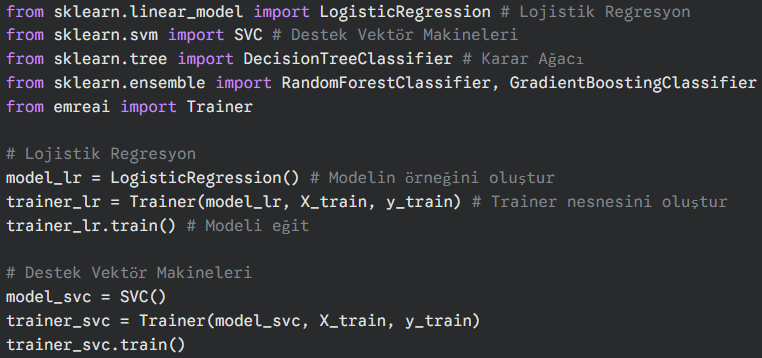
\includegraphics[scale=0.500]{figure6.png}
  \caption{\textsc{Scikit-learn Models}}
\end{figure}

EmreAI also provides integration for training deep learning models with \texttt{TensorFlow/Keras}.

\begin{figure}[htbp]
  \centering
  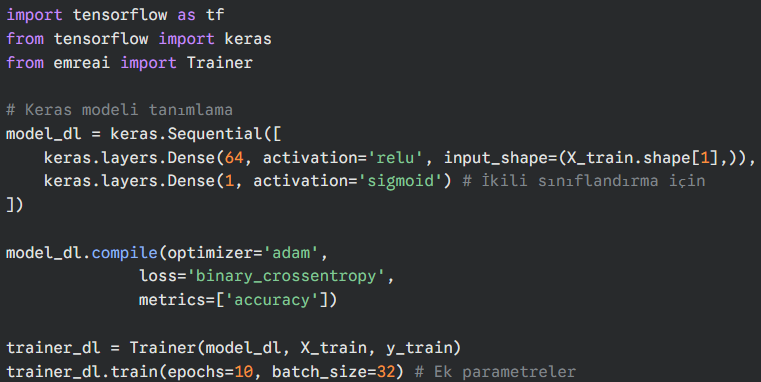
\includegraphics[scale=0.500]{figure7.png}
  \caption{\textsc{TensorFlow/Keras Models}}
\end{figure}

A Keras model is defined, compiled using the \texttt{compile()} method, and trained using \texttt{Trainer}. The \texttt{train()} method can accept additional parameters such as \texttt{epochs} (number of training iterations) and \texttt{batch\_size} (mini-batch size).

\subsection{Saving and Loading Models}

Saving and loading a trained machine learning model is a crucial step to enable its reuse without retraining. EmreAI provides simple and effective methods for this process.

The method for saving a model depends on the machine learning library used (\texttt{scikit-learn}, \texttt{TensorFlow}, \texttt{PyTorch}).

\texttt{Scikit-learn} models can be saved using \texttt{joblib} or \texttt{pickle}. \texttt{joblib} is more efficient for models containing large \texttt{NumPy} arrays.

To save a model, use the following command:
\texttt{joblib.dump(model, 'model.joblib')}

\texttt{TensorFlow}/\texttt{Keras} models are saved using the \texttt{model.save()} method. This method saves the model's architecture, weights, and optimization state.

To save a model, use the following command:
\texttt{model.save('model')} or \texttt{model.save('model.h5')}

\texttt{PyTorch} models save the model's \texttt{state\_dict}, which contains the learned parameters (weights and biases).

To save a model, use the following command:
\texttt{torch.save(model.state\_dict(), 'model.pth')}

Saved models can easily be loaded later for use.

To load a model, use the following methods:
\begin{footnotesize}
\begin{itemize}
    \item For \texttt{Scikit-learn}: \texttt{model = joblib.load('model.joblib')}
    \item For \texttt{TensorFlow}/\texttt{Keras}: \texttt{model = tf.keras.models.load\_model('model')}
    \item For \texttt{PyTorch}: First, create the model architecture, then load the saved \texttt{state\_dict}:
    \begin{verbatim}
    model = Net(input_dim)
    model.load_state_dict(torch.load('model.pth'))
    \end{verbatim}
\end{itemize}
\end{footnotesize}

\section{Conclusion}

In this study, the challenges encountered in the development and deployment processes of data science and machine learning projects, as well as the solutions offered by the EmreAI framework to address these challenges, are comprehensively examined. Specifically, the integration issues, complex and repetitive workflows, code duplication, and the need to convert data formats between different tools arising from the separate use of various data processing tools (such as Pandas, NumPy, etc.) and machine learning/deep learning frameworks (such as TensorFlow, PyTorch, Scikit-learn, etc.) are explored in detail. The fragmented nature of the current data science ecosystem causes data scientists to spend a significant portion of their time on infrastructure management and integration issues, hindering the focus on model development and problem-solving processes.

In response to the challenges posed by the fragmented nature of the current data science ecosystem, the EmreAI framework offers significant advantages by integrating the entire machine learning workflow from data acquisition to model deployment into a single platform. This integration eliminates the need for transitioning between different tools and converting data formats, significantly simplifying and accelerating workflows. The paper provides a detailed explanation of EmreAI's core features and architecture, along with Python code examples demonstrating how these features can be practically applied. These examples are crucial in showing how EmreAI can be adapted to different use cases and offer solutions to real-world problems.

The key features of EmreAI highlighted and discussed in the study are summarized as follows:

\textbf{Unified Workflow Integration}: EmreAI offers a fully integrated solution encompassing all stages of the machine learning process, including data acquisition, preprocessing, model training, hyperparameter optimization, model evaluation, and deployment. This integration eliminates the need for switching between different tools and converting data formats, greatly simplifying the workflow and enabling data scientists to focus more on model development and problem-solving. As a result, project development times are shortened, and productivity increases.
  
\textbf{Modular Design: }EmreAI's modular architecture provides high flexibility, reusability, and ease of extensibility by treating each step (such as data preprocessing, modeling, optimization, deployment, etc.) as independent modules. This modular structure allows for easy integration of new algorithms, data processing techniques, or deployment methods into the system. Additionally, it enables the creation of customized workflows based on different project requirements. For example, various text preprocessing steps or image augmentation techniques can be easily added to the system.

\textbf{Hybrid Backend Support:} EmreAI's support for both CPU and GPU, along with integration with popular cloud platforms such as AWS, GCP, and Azure, ensures that it has a scalable and flexible infrastructure. This feature makes EmreAI an ideal solution for projects with different hardware and infrastructure requirements. The use of cloud-based resources, particularly when working with large datasets and complex models, significantly enhances performance.

\textbf{AutoML and Hyperparameter Tuning:} With its built-in AutoML engine, which includes advanced hyperparameter optimization algorithms such as Bayesian optimization, genetic algorithms, and PBT, EmreAI automatically achieves optimal model performance. This feature eliminates the need for manual hyperparameter tuning, saving time and helping to achieve better model performance. Integration with powerful optimization tools such as Optuna, Ray Tune, and Hyperopt makes it easier to try and compare different optimization strategies.

\textbf{Reproducibility and Experiment Management:} EmreAI offers integration with tools like MLflow and DVC (Data Version Control) to ensure the reproducibility and traceability of experiments and results. This feature enhances the transparency, reliability, and auditability of data science projects. Versioning of experiments, recording parameters and metrics, and comparing different runs make it easier to select the best model. DVC integration provides significant advantages in data management and model reproducibility by enabling data and model versioning.

\textbf{Deployment-Ready APIs:} EmreAI facilitates the creation of RESTful APIs for trained models, simplifying the integration of models into web applications, mobile apps, IoT devices, or other systems. This feature enables the quick and efficient deployment of models into production environments.

\textbf{Explainable AI (XAI)}: Integration with XAI techniques such as SHAP, LIME, and Grad-CAM enables understanding and interpreting how model predictions are made. This increases the reliability of the model and provides transparency, especially in critical decision-making processes.

\textbf{Scalable Data Management:}EmreAI integrates with technologies like Apache Arrow, Parquet, Dask, and Spark, enabling efficient handling of large datasets. This ensures that EmreAI can be used with high performance in big data projects and supports the scalability of data processing workflows.

The study also provides detailed examples demonstrating how EmreAI processes various types of data (CSV, text, images, time series, etc.) and applies suitable preprocessing techniques (such as handling missing data, feature scaling, text cleaning, TF-IDF vectorization, image resizing, normalization, time series decomposition, etc.) for these data types.

In conclusion, the EmreAI framework is a powerful and integrated tool that reduces the complexity of the development and deployment processes in modern data science and machine learning projects, significantly accelerating these processes. With features such as unified workflow integration, modular design, hybrid backend support, AutoML capabilities, experiment management, easy API creation, XAI integration, and scalable data management, EmreAI allows data scientists to work more efficiently and achieve better results in a shorter time. In the future, EmreAI is expected to support more data types, preprocessing techniques, model architectures, optimization algorithms, and deployment options, offer specialized modules for various ML domains (such as natural language processing, computer vision, etc.), and feature an even more user-friendly interface. With these enhancements, EmreAI is anticipated to be widely adopted by a broader user base and play a significant role in the field of data science and machine learning. In particular, the proliferation of integrated platforms like EmreAI is expected to contribute to the increased accessibility of artificial intelligence and machine learning technologies, accelerating their applications across various industries.


% An example of a floating figure using the graphicx package.
% Note that \label must occur AFTER (or within) \caption.
% For figures, \caption should occur after the \includegraphics.
% Note that IEEEtran v1.7 and later has special internal code that
% is designed to preserve the operation of \label within \caption
% even when the captionsoff option is in effect. However, because
% of issues like this, it may be the safest practice to put all your
% \label just after \caption rather than within \caption{}.
%
% Reminder: the "draftcls" or "draftclsnofoot", not "draft", class
% option should be used if it is desired that the figures are to be
% displayed while in draft mode.
%
%\begin{figure}[!t]
%\centering
%\includegraphics[width=2.5in]{myfigure}
% where an .eps filename suffix will be assumed under latex,
% and a .pdf suffix will be assumed for pdflatex; or what has been declared
% via \DeclareGraphicsExtensions.
%\caption{Simulation Results}
%\label{fig_sim}
%\end{figure}

% Note that IEEE typically puts floats only at the top, even when this
% results in a large percentage of a column being occupied by floats.

% An example of a double column floating figure using two subfigures.
% (The subfig.sty package must be loaded for this to work.)
% The subfigure \label commands are set within each subfloat command, the
% \label for the overall figure must come after \caption.
% \hfil must be used as a separator to get equal spacing.
% The subfigure.sty package works much the same way, except \subfigure is
% used instead of \subfloat.
%
%\begin{figure*}[!t]
%\centerline{\subfloat[Case I]\includegraphics[width=2.5in]{subfigcase1}%
%\label{fig_first_case}}
%\hfil
%\subfloat[Case II]{\includegraphics[width=2.5in]{subfigcase2}%
%\label{fig_second_case}}}
%\caption{Simulation results}
%\label{fig_sim}
%\end{figure*}
%
% Note that often IEEE papers with subfigures do not employ subfigure
% captions (using the optional argument to \subfloat), but instead will
% reference/describe all of them (a), (b), etc., within the main caption.


% An example of a floating table. Note that, for IEEE style tables, the
% \caption command should come BEFORE the table. Table text will default to
% \footnotesize as IEEE normally uses this smaller font for tables.
% The \label must come after \caption as always.
%
%\begin{table}[!t]
%% increase table row spacing, adjust to taste
%\renewcommand{\arraystretch}{1.3}
% if using array.sty, it might be a good idea to tweak the value of
% \extrarowheight as needed to properly center the text within the cells
%\caption{An Example of a Table}
%\label{table_example}
%\centering
%% Some packages, such as MDW tools, offer better commands for making tables
%% than the plain LaTeX2e tabular which is used here.
%\begin{tabular}{|c||c|}
%\hline
%One & Two\\
%\hline
%Three & Four\\
%\hline
%\end{tabular}
%\end{table}


% Note that IEEE does not put floats in the very first column - or typically
% anywhere on the first page for that matter. Also, in-text middle ("here")
% positioning is not used. Most IEEE journals/conferences use top floats
% exclusively. Note that, LaTeX2e, unlike IEEE journals/conferences, places
% footnotes above bottom floats. This can be corrected via the \fnbelowfloat
% command of the stfloats package.


% use section* for acknowledgement
%\section*{TEŞEKKÜR}
%Yazarın teşekkür etmek istediği kurum yada kişiler burada belirtilecek.
\section*{ACKNOWLEDGMENTS}
The author would like to express sincere gratitude to Olcay Taner Yıldız for his invaluable support and guidance throughout this work. His insightful advice, constructive feedback, and continuous encouragement played a significant role in the success of this project. The author is deeply appreciative of his willingness to share his expertise and time, which greatly contributed to the development of this research.


% trigger a \newpage just before the given reference
% number - used to balance the columns on the last page
% adjust value as needed - may need to be readjusted if
% the document is modified later
%\IEEEtriggeratref{8}
% The "triggered" command can be changed if desired:
%\IEEEtriggercmd{\enlargethispage{-5in}}

% references section

% can use a bibliography generated by BibTeX as a .bbl file
% BibTeX documentation can be easily obtained at:
% http://www.ctan.org/tex-archive/biblio/bibtex/contrib/doc/
% The IEEEtran BibTeX style support page is at:
% http://www.michaelshell.org/tex/ieeetran/bibtex/
%\bibliographystyle{IEEEtran}
% argument is your BibTeX string definitions and bibliography database(s)
%\bibliography{IEEEabrv,../bib/paper}
%
% <OR> manually copy in the resultant .bbl file
% set second argument of \begin to the number of references
% (used to reserve space for the reference number labels box)
\renewcommand{\refname}{References}
\begin{thebibliography}{1}

\bibitem{paper1}
Rajkomar, A.; Dean, J.; Kohane, I. Machine learning in medicine. N. Engl. J. Med. 2019, 380, 1347–1358.

\bibitem{paper2}
Enughwure, A.; Febaide, I. Applications of Artificial Intelligence in Combating COVID-19: A Systematic Review. Open Access Libr. J. 2020, 7, 1–12.


\bibitem{paper3}
Carleo, G.; Cirac, I.; Cranmer, K.; Daudet, L.; Schuld, M.; Tishby, N.; Vogt-Maranto, L.; Zdeborová, L. Machine learning and the physical sciences. Rev. Mod. Phys. 2019, 91, 045002. 


\bibitem{paper4}
eCun, Y., Bengio, Y., Hinton, G. (2015). Deep Learning. Nature, 521(7553), 436-444. 

\bibitem{paper5}
DAI, H., PENG, X., SHI, X., HE, L., XIONG, Q., JIN, H. (2021). Reveal training performance mystery between TensorFlow and PyTorch in the single GPU environment. Science China Information Sciences, 65(1), 112103:1–112103:17. 

\bibitem{paper6}
Martín Abadi, Paul Barham, Jianmin Chen, Zhifeng Chen, Andy Davis, Jeffrey Dean, Matthieu Devin, Sanjay Ghemawat, Geoffrey
Irving, Michael Isard, Manjunath Kudlur, Josh Levenberg, Rajat Monga, Sherry Moore, Derek G. Murray, Benoit Steiner, Paul Tucker,
Vijay Vasudevan, Pete Warden, Martin Wicke, Yuan Yu, and Xiaoqiang Zheng. 2016. TensorFlow: A System for Large-Scale Machine
Learning. In Proceedings of the 12th USENIX Conference on Operating Systems Design and Implementation (Savannah, GA, USA) (OSDI
’16). USENIX Association, USA, 265–283.

\bibitem{paper7}
Adam Paszke, Sam Gross, Francisco Massa, Adam Lerer, James Bradbury, Gregory Chanan, Trevor Killeen, Zeming Lin, Natalia
Gimelshein, Luca Antiga, Alban Desmaison, Andreas Kopf, Edward Yang, Zachary DeVito, Martin Raison, Alykhan Tejani, Sasank
Chilamkurthy, Benoit Steiner, Lu Fang, Junjie Bai, and Soumith Chintala. 2019. PyTorch: An Imperative Style, High-Performance Deep
Learning Library. In Advances in Neural Information Processing Systems 32 (NeurIPS). Curran Associates, Inc., 8024–8035.

\bibitem{paper8}
Novac, O.-C., Chirodea, M. C., Novac, C. M., Bizon, N., Oproescu, M., Stan, O. P.,Gordan, C. E. (2022). Analysis of the application efficiency of TensorFlow and PyTorch in convolutional neural network. Sensors, 22(22), 8872

\bibitem{paper9}
Smith, J., Brown, K., Wilson, R. (2018). Comparative Analysis of Deep Learning Frameworks. Journal of Machine Learning Research, 19, 1-27. 

\bibitem{paper10}
Chen, Y., Wan, Z., Zhuang, Y., Liu, N., Lo, D.,Yang, X. (n.d.). *Understanding the OSS Communities of Deep Learning Frameworks: A Comparative Case Study of PyTorch and TensorFlow. The State Key Laboratory of Blockchain and Data Security, Zhejiang University, China; City University of Hong Kong, Hong Kong; Singapore Management University, Singapore.

\bibitem{paper11}
Yapıcı, M. Mutlu, and Topaloğlu, N. (2021). "Performance comparison of deep learning frameworks." *Computers and Informatics*, 2757-8259, Volume 1 Issue 1.

\bibitem{paper12}
Paszke, A.; Gross, S.; Massa, F.; Lerer, A.; Bradbury, J.; Chanan, G.; Killeen, T.; Lin, Z.; Gimelshein, N.; Antiga, L.; et al. Pytorch: An Imperative Style, High-Performance Deep Learning Library. In Advances in Neural Information Processing Systems; Curran Associates, Inc.: Red Hook, NY, USA, 2019; Volume 32, pp. 8024–8035. 


\bibitem{paper13}
Goodfellow, I., Bengio, Y.,Courville, A. (2016). Deep Learning. MIT Press.

\bibitem{paper14}
Abadi, M.; Barham, P.; Chen, J.; Chen, Z.; Davis, A.; Dean, J.; Devin, M.; Ghemawat, S.; Irving, G.; Isard, M.; et al. Tensorflow: A system for large-scale machine learning. In Proceedings of the 12th USENIX Conference on Operating Systems Design and Implementation, Savannah, GA, USA, 2–4 November 2016; pp. 265–283.

\bibitem{paper15}
Liang, X., Zhang, C.,Wang, T. (2019). Optimizing Machine Learning Frameworks: A Comparative Study. IEEE Transactions on Neural Networks and Learning Systems, 30(4), 1235-1248.


\bibitem{paper16}
Molnar, C. (2022). Interpretable Machine Learning: A Guide for Making Black Box Models Explainable. Lulu Press, Inc.

\end{thebibliography}


% that's all folks
\end{document}